\documentclass[sn-mathphys-ay]{sn-jnl}

% -------------------------------------------------
% Packages
% -------------------------------------------------
\usepackage{amsmath,amssymb,amsthm,mathtools}
\usepackage{bm}
\usepackage{booktabs}
\usepackage{graphicx}
\usepackage{multirow}
\usepackage{array}
\usepackage{enumitem}
\usepackage{xurl}
\usepackage{hyperref}
\usepackage{doi}
\Urlmuskip=0mu plus 1mu\relax
\raggedbottom
\hbadness=10000
\vbadness=10000

% -------------------------------------------------
% Theorem environments
% -------------------------------------------------
\theoremstyle{plain}
\newtheorem{assumption}{Assumption}
\newtheorem{lemma}{Lemma}
\newtheorem{proposition}{Proposition}
\newtheorem{corollary}{Corollary}
\newtheorem{theorem}{Theorem}

\theoremstyle{remark}
\newtheorem{remark}{Remark}

% -------------------------------------------------
% Macros
% -------------------------------------------------
\newcommand{\R}{\mathbb{R}}
\newcommand{\argmax}{\operatornamewithlimits{argmax}}
\newcommand{\argmin}{\operatornamewithlimits{argmin}}

\begin{document}

\title[Participation Capacity and Standards Blocs]{Participation Capacity, Standards Blocs, and Inefficient International Standardization}

\author*{\fnm{Ryota} \sur{Matsuki}}\email{ryota.matsuki@gmail.com}

\affil{\orgname{Independent Researcher},
  \orgaddress{\city{Matsuyama}, \state{Ehime}, \country{Japan}}}

\abstract{
This paper develops a three-country model of international standardization with network externalities, coalition formation, and asymmetric participation capacity. Countries choose among a standards war, a two-country standardization union, and full international standardization. Mutual recognition removes the baseline technology-gap cost within the recognition area, but countries may still face residual compliance costs because they differ in their ability to comply with, test, certify, and implement the common standard. The model therefore distinguishes formal accession from effective participation.

The analysis yields three main results. First, full international standardization may maximize world welfare without arising in equilibrium. A low-capacity outsider may contribute too little to the common installed base, relative to the additional competitive pressure its accession creates in incumbent-member markets, for accession to be privately attractive. Second, stronger network effects do not necessarily favor full harmonization uniformly. On a verified parameter region with pronounced participation-capacity asymmetry, stronger network effects can instead stabilize an exclusionary two-country standards bloc. Third, once participation capacity is endogenized, capacity-building investment and conditional transfer policy can, on a verified compact domain for the policy analysis, restore the accession margin more effectively than policies that merely preserve fragmented national standards.

The results suggest that inefficient fragmentation may persist not only because of strategic exclusion, but also because weaker participants cannot translate formal recognition into effective market integration.

\medskip
\noindent\textit{JEL codes:} F13, L13, L15, O33.
}

\keywords{international standardization\enspace$\cdot$\enspace network externalities\enspace$\cdot$\enspace compatibility\enspace$\cdot$\enspace standards bloc\enspace$\cdot$\enspace participation capacity\enspace$\cdot$\enspace mutual recognition}

\setlength{\emergencystretch}{2em}
\maketitle

% =================================================
% Section 1
% =================================================
\section{Introduction}

Technical standards are fundamental to the organization of markets. By shaping compatibility, interoperability, and the size of the installed base, standards affect firms' incentives to innovate, consumers' adoption decisions, and the intensity of product-market competition. The classic literature in industrial organization has shown that network externalities may generate coordination failures, excess inertia, inefficient standardization, and ambiguous welfare effects of compatibility \citep{FarrellSaloner1985,KatzShapiro1985,KatzShapiro1986,FarrellSaloner1986,KatzShapiro1992,KatzShapiro1994}. More broadly, standards influence industry structure and economic performance through entry conditions, product variety, technological progress, and the allocation of market power \citep{DavidGreenstein1990,MatutesRegibeau1996,Shy2001,BesenFarrell1994,Tassey2017}.

These issues become even more consequential in an international setting. When standards differ across countries, firms face adaptation and compliance costs in foreign markets, and governments must decide whether to preserve national standards, recognize foreign standards, or participate in broader harmonization arrangements. A strand of the international trade literature has therefore analyzed standard recognition, mutual recognition, and strategic incompatibility as policy choices rather than purely technological facts \citep{GandalShy2001,BarrettYang2001,Costinot2008,Klimenko2009}. In particular, \citet{GandalShy2001} show that governments may have incentives to form standardization unions when network effects and conversion costs interact, while \citet{BarrettYang2001}, \citet{Costinot2008}, and \citet{Klimenko2009} emphasize that institutional design---including incompatibility, national treatment, interoperability, and mutual recognition---can systematically alter equilibrium standards and welfare. The coalition-formation aspect of this problem is also structurally related to trade-agreement models with insider-outsider tensions \citep{Riezman1985,Krishna1998}, although the object of negotiation here is standard recognition rather than tariffs.

At the same time, the economics of standards has expanded well beyond the older compatibility-versus-variety trade-off. Recent work increasingly treats standards as part of the infrastructure of innovation, regulation, and international market access. Standards and regulation affect innovation differently across market environments \citep{BlindPetersenRiillo2017}; technology standards can alter firms' product-innovation incentives \citep{FoucartLi2021}; and participation in formal standardization processes is itself shaped by strategic and institutional determinants \citep{BlindVonLaer2022,BlindKenneyLeiponenSimcoe2023}. On the trade side, empirical studies show that international standards and standard harmonization can promote cross-border exchange and market integration \citep{CloughertyGrajek2014,SchmidtSteingress2022}. More recent evidence also links international standards to export performance and innovation outcomes in a globalizing economy \citep{BlindMuench2024,WangZhu2025}. In parallel, new data efforts such as StanDat are lowering the empirical barriers to studying international standards, participation patterns, and cross-country standardization behavior \citep{Bjorkholt2026}.

A complementary institutional motivation comes from the literature on mutual
recognition agreements (MRAs), the WTO/TBT framework, and developing-country
participation in standardization \citep{WTO_TBT,ISO_UNIDO}. Those literatures
emphasize that formal recognition and market access often depend not only on
nominal membership in a common standards architecture, but also on testing
capability, certification infrastructure, regulatory implementation, and
effective participation in conformity-assessment systems. This paper abstracts
from those institutional details, but its participation-capacity parameter is
designed precisely to capture the residual compliance burden that remains when
formal recognition is granted but effective participation is incomplete. In
that sense, the model connects the compatibility literature to the
institutional question of why mutual recognition may fail to deliver fully
integrated standardization outcomes in practice.

Despite this broad and growing literature, one feature remains underexplored in formal models of international standardization. Much of the existing theory effectively treats accession to a common standard as removing the relevant cross-border friction once recognition is granted. In practice, however, formal accession and effective participation need not coincide. Countries differ not only in whether they are legally admitted to a harmonized regime, but also in whether firms can actually comply with, test, certify, and implement the standard at low cost. This distinction is particularly important when standardization is mediated by mutual recognition or bloc formation. A country may formally join a standard area yet remain a weak participant because residual compliance burdens continue to limit its contribution to the common installed base and its competitive presence in foreign markets. While the existing literature has rich insights on compatibility, standard recognition, and institutional design \citep{FarrellSaloner1985,KatzShapiro1985,GandalShy2001,BarrettYang2001,Costinot2008,Klimenko2009}, comparatively less attention has been paid to how \emph{participation-capacity asymmetry} interacts with network externalities and coalition formation in a multi-country setting.

This paper develops a simple three-country model to study that issue. The framework builds on the standards-war versus harmonization logic in the compatibility literature \citep{FarrellSaloner1985,KatzShapiro1985,KatzShapiro1986,KatzShapiro1994} and on the international standardization setting of \citet{GandalShy2001}, but introduces country-specific participation capacity. Three countries, each with one firm, choose among three regimes: a standards war ($SW$), a two-country standardization union ($SU$), and full international standardization ($IS$). Mutual recognition removes the baseline technology-gap cost inside the recognition area, but countries may still face residual compliance costs because participation capacity differs across them. In this environment, formal membership in a common standard and effective participation in that standard are distinct objects.

The model delivers three main results. First, full international standardization may maximize world welfare while failing to arise in equilibrium, because a low-capacity outsider contributes too little to the common installed base relative to the additional competitive pressure its accession creates in member-country markets. Second, stronger network effects need not monotonically favor full harmonization: over a verified parameter region with sufficiently pronounced participation-capacity asymmetry, stronger network effects can instead stabilize an exclusionary two-country standards bloc. Third, once participation capacity is endogenized, capacity-building policies and conditional transfers targeted at the low-capacity country can, on the verified compact domain used in Section~5, restore the accession margin more effectively than policies that merely preserve fragmented national standards. In that sense, the paper shifts attention from formal recognition alone to the deeper question of whether countries are able to participate effectively in a harmonized regime.

These results contribute to the literature in three ways. Relative to the classic compatibility literature, the paper introduces a tractable distinction between formal compatibility and effective participation \citep{FarrellSaloner1985,KatzShapiro1985,KatzShapiro1986,DavidGreenstein1990}. Relative to the international standardization literature, it shows how residual post-accession frictions can sustain inefficient exclusion even when mutual recognition is technologically feasible \citep{GandalShy2001,BarrettYang2001,Costinot2008,Klimenko2009}. Relative to recent empirical work on standards, trade, and innovation, it offers a mechanism through which participation asymmetries can shape the formation and persistence of standards blocs \citep{BlindPetersenRiillo2017,FoucartLi2021,BlindVonLaer2022,BlindKenneyLeiponenSimcoe2023,CloughertyGrajek2014,SchmidtSteingress2022,BlindMuench2024,WangZhu2025,Bjorkholt2026}. The resulting perspective is useful for interpreting why harmonization may fail not only because of strategic exclusion, but also because weaker participants lack the capacity to translate formal accession into effective market integration.

The policy implication is straightforward, though Section~5 makes clear that it is conditional on additional monotonicity assumptions. If fragmentation persists because low-capacity countries cannot participate effectively in a harmonized regime, then the relevant policy margin is not merely whether formal recognition is granted, but whether participation capacity can be improved. This insight links the paper's theory to contemporary discussions of standardization as part of broader innovation and regulatory infrastructure \citep{Tassey2017,BlindPetersenRiillo2017,BlindKenneyLeiponenSimcoe2023,BlindMuench2024}. In the model, targeted capacity-building and conditional transfer policies relax the actual bottleneck in the regime-selection game, whereas policies that simply preserve separate national standards do not.

The remainder of the paper is organized as follows. Section~2 presents the model. Section~3 derives firm equilibrium under $SW$, $SU$, and $IS$. Section~4 characterizes governments' regime choices under participation-capacity asymmetry. Section~5 endogenizes participation capacity through investment and studies conditional transfer policy. Section~6 concludes.


% =================================================
% Section 2
% =================================================
\section{Model}

We consider three countries, indexed by $k \in K \equiv \{A,B,C\}$. Each country has a single domestic firm, also indexed by $k$. Markets are segmented: firms can sell in all three countries, but consumers in country $k$ purchase only in market $k$. Competition in each market is \`a la Cournot.

The model preserves the three-regime structure of the original framework---a standards war, a two-country standardization union, and full international standardization---but introduces asymmetry in \emph{participation capacity}. Participation capacity captures a country's ability to comply with, test, certify, and implement a mutually recognized standard. This is the new friction that distinguishes the present model from the benchmark.

\subsection{Standardization regimes}

Each country initially has its own national standard. We consider three possible regimes.

\begin{enumerate}
    \item \textbf{Standards War (SW).} All countries keep their own standards and no mutual recognition takes place.
    \item \textbf{Standardization Union (SU).} Countries $A$ and $B$ mutually recognize each other's standards, while country $C$ remains outside the union.
    \item \textbf{International Standardization (IS).} All three countries mutually recognize a common standard.
\end{enumerate}

Let $r \in \{SW,SU,IS\}$ denote the regime. For each regime $r$, let $G_r(i)$ denote the recognition group to which firm $i$ belongs. Thus,
\[
G_{SW}(A)=\{A\},\quad G_{SW}(B)=\{B\},\quad G_{SW}(C)=\{C\},
\]
\[
G_{SU}(A)=G_{SU}(B)=\{A,B\},\quad G_{SU}(C)=\{C\},
\]
and
\[
G_{IS}(A)=G_{IS}(B)=G_{IS}(C)=\{A,B,C\}.
\]

\subsection{Consumers and demand}

Demand is derived from a quasi-linear representative-consumer utility in each market. Let $q_{ik}^r$ denote consumption of the variety supplied by firm $i$ in market $k$ under regime $r$, and let
\[
Q_k^r \equiv \sum_{i \in K} q_{ik}^r
\]
be total quantity sold in market $k$.

For any recognition group $g \subseteq K$, define the compatible installed base under regime $r$ by
\[
N_g^r \equiv \sum_{m \in K} \sum_{j \in g} q_{jm}^r.
\]
Positive network effects arise only when at least two countries belong to the same recognition group. Hence define
\[
B_g^r \equiv 
\begin{cases}
N_g^r & \text{if } |g| \ge 2,\\
0   & \text{if } |g| = 1.
\end{cases}
\]

Let $v \ge 0$ denote the strength of the network externality. In market $k$ under regime $r$, the representative consumer has utility
\begin{equation}
U_k^r(\{q_{ik}^r\}_{i \in K})
=
\sum_{i \in K} \bigl(1 + v B_{G_r(i)}^r\bigr) q_{ik}^r
-
\frac{1}{2}(Q_k^r)^2
-
\sum_{i \in K} p_{ik}^r q_{ik}^r.
\label{eq:utility}
\end{equation}
Maximization of \eqref{eq:utility} with respect to each $q_{ik}^r$ yields the inverse demand for firm $i$ in market $k$:
\begin{equation}
p_{ik}^r = 1 - Q_k^r + v B_{G_r(i)}^r.
\label{eq:inverse_demand}
\end{equation}

Equation \eqref{eq:inverse_demand} is therefore a linear-quadratic demand
system with a common congestion term $Q_k^r$ and firm-specific intercept
shifters determined by compatible installed bases. A larger compatible
installed base shifts outward the demand for firms belonging to the same
recognized standard area. Under $SW$, no such benefit arises because each
country remains isolated. Under $SU$, firms $A$ and $B$ benefit from a common
installed base, while firm $C$ does not. Under $IS$, all firms benefit from the
same installed base.

\subsection{Technology gap and participation capacity}

Each domestic firm can produce for its home market at zero marginal cost. Supplying a foreign market is costly for two distinct reasons.

First, there is a \emph{technology-gap cost} $c>0$, which captures the baseline adaptation cost when a firm must supply a market governed by a non-recognized foreign standard.

Second, there is a country-specific \emph{participation-capacity friction}. Let $\theta_k \in [0,1]$ denote country $k$'s participation capacity. A higher $\theta_k$ means that firms from country $k$ can more easily comply with, test, and certify goods under a mutually recognized standard. The residual compliance cost is
\begin{equation}
\tau_k \equiv \mu(1-\theta_k), \qquad \mu>0.
\label{eq:tau}
\end{equation}

We assume that countries $A$ and $B$ are ex ante symmetric and have relatively high participation capacity, whereas country $C$ is less capable:
\begin{equation}
\bar\theta_A=\bar\theta_B>\bar\theta_C.
\label{eq:theta_order}
\end{equation}

Given regime $r$, the marginal cost of firm $i$ when selling in market $k$ is
\begin{equation}
m_{ik}^r=
\begin{cases}
0 & \text{if } i=k,\\[4pt]
\tau_i & \text{if } i\neq k \text{ and } k \in G_r(i),\\[4pt]
c+\tau_i & \text{if } i\neq k \text{ and } k \notin G_r(i).
\end{cases}
\label{eq:marginal_cost}
\end{equation}

Equation \eqref{eq:marginal_cost} is the key extension. If countries mutually recognize one another's standards, the technology-gap component $c$ is removed within that recognition area, but the residual compliance burden $\tau_i$ remains unless participation capacity is perfect. When $\theta_i=1$, we have $\tau_i=0$, so the model nests the benchmark in which mutual recognition completely eliminates cross-border adaptation costs.

The reduced-form specification in \eqref{eq:tau} should be interpreted as an
exporter-side index of effective standard-participation capability. It bundles
together the ability to test, certify, document, implement, and adapt to a
common standard in foreign markets. Accordingly, the residual compliance cost
$\tau_i$ is not meant to represent a single technological friction, but rather
a composite conformity-assessment and implementation burden that remains even
after formal recognition is granted. Destination-country institutions still
matter, but in the present model they are absorbed into the regime definition
and the baseline technology-gap cost $c$: within a recognition area, all
exporters face the same legal treatment in the destination market, while
$\tau_i$ captures how effectively exporters from country $i$ can take advantage
of that treatment. A bilateral version of this friction would also be natural,
but the exporter-specific summary keeps the model tractable and allows the
analysis to focus sharply on the accession margin. The asymmetry of interest is
therefore exporter-specific rather than destination-specific.

Although the model is theoretical, its parameters admit a natural empirical
interpretation. The technology-gap term $c$ can be read as a reduced-form
summary of the baseline cost of operating across distinct standards
architectures, while the residual compliance term $\tau_i$ captures the
exporter-side burden associated with testing, certification, documentation, and
implementation under a formally recognized standard. In this sense, a larger
$\tau_C$ corresponds to a country that has nominal access to a common standard
but remains weakly integrated into its conformity-assessment and implementation
system. The parameter domains studied below should therefore be interpreted as
stylized policy regions rather than as literal calibrated estimates.

Firm $i$'s profit under regime $r$ is
\begin{equation}
\pi_i^r = \sum_{k \in K} \left(p_{ik}^r - m_{ik}^r\right) q_{ik}^r.
\label{eq:profit}
\end{equation}

At stage 4, firms simultaneously choose quantities in each market to maximize \eqref{eq:profit}, taking the regime and participation capacities as given.

Figure~\ref{fig:regime_schematic} visualizes the distinction between formal
recognition and effective participation that drives the model.

\begin{figure}[t]
\centering
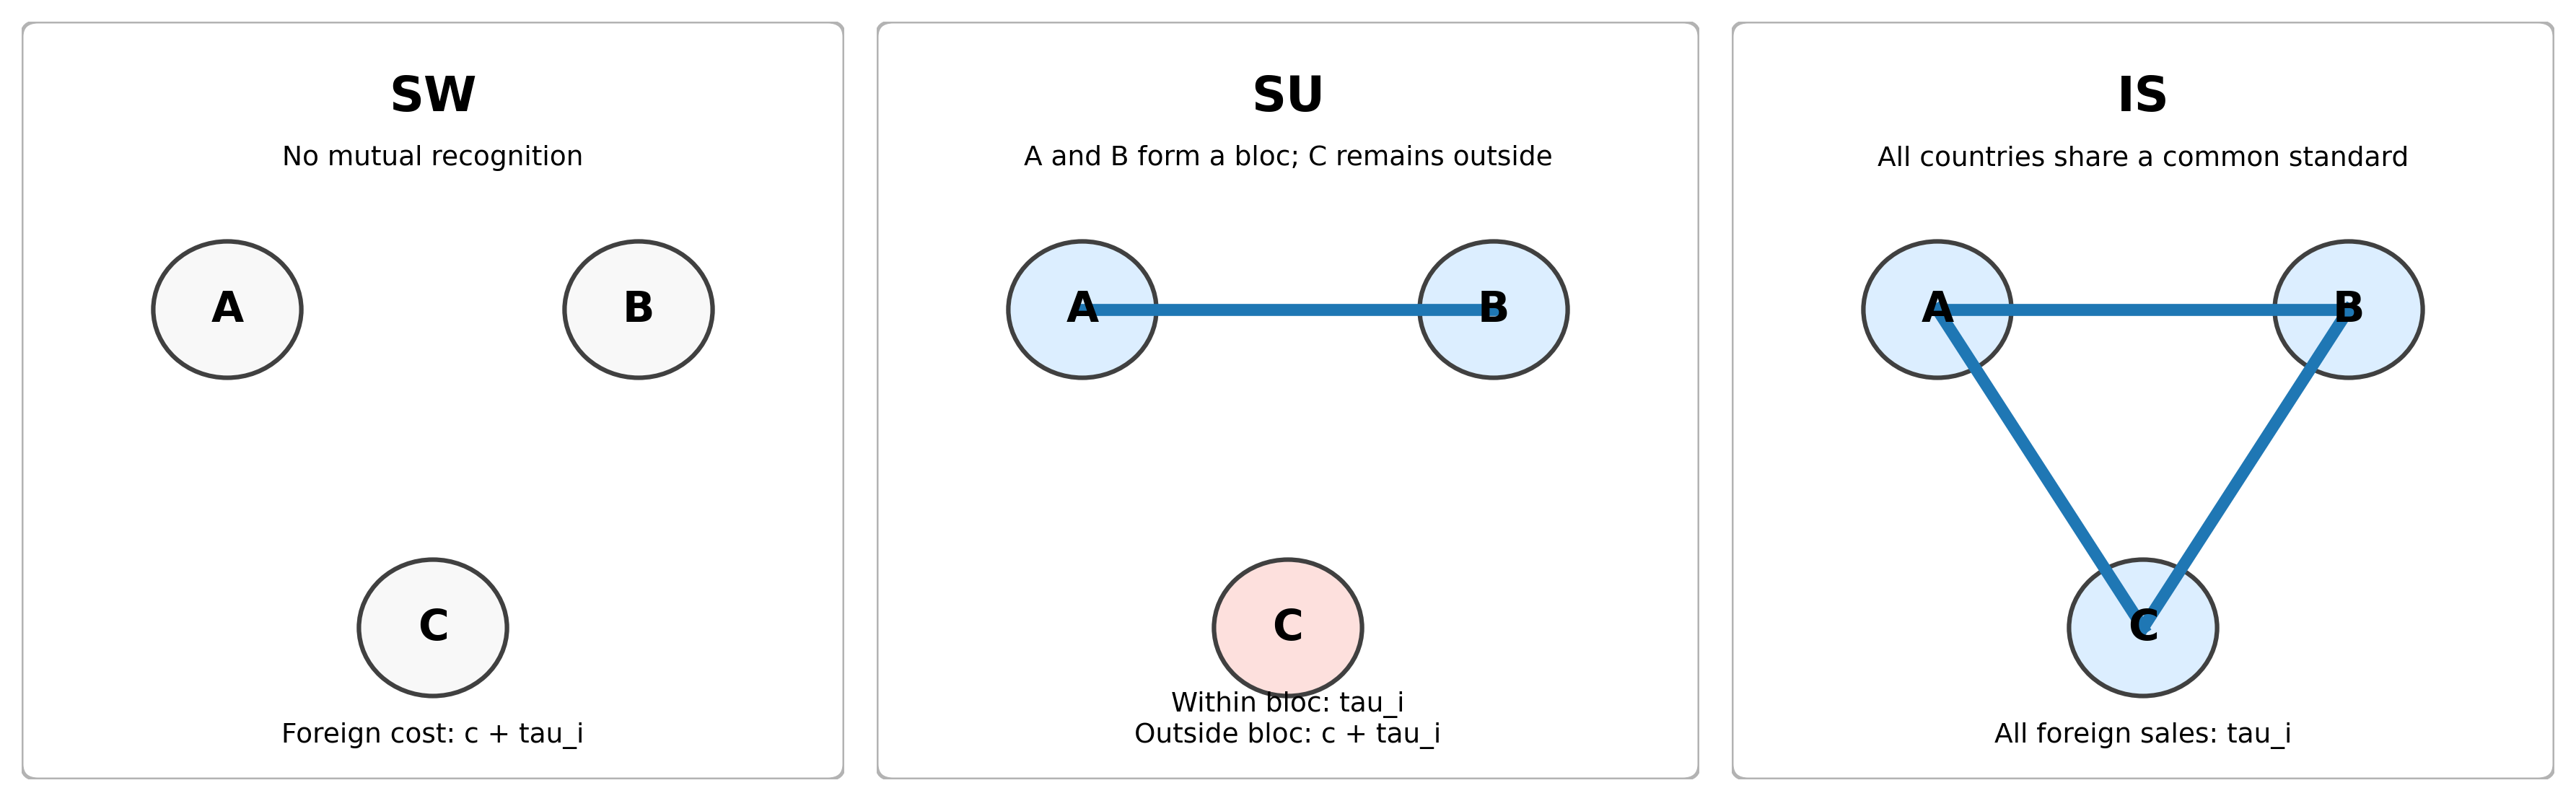
\includegraphics[width=.92\linewidth]{figures/fig1_regime_schematic.png}
\caption{Standardization regimes and residual compliance costs. The figure illustrates how foreign-market marginal costs differ across the three regimes. Under $SW$, all foreign sales incur the baseline technology-gap cost plus the exporter-specific residual compliance cost, $c+\tau_i$. Under $SU$, sales within the member bloc avoid the technology-gap component and incur only $\tau_i$, whereas sales to or from the outsider still incur $c+\tau_i$. Under $IS$, mutual recognition removes the technology-gap component in all foreign markets, but exporter-specific residual compliance costs remain unless participation capacity is perfect.}
\label{fig:regime_schematic}
\end{figure}

\subsection{Capacity investment}

To give participation capacity a policy interpretation, we endogenize it.
Before any standardization decision is made, government $k$ chooses capacity
investment $I_k \ge 0$, subject to
\[
I_k \in [0,1-\bar\theta_k].
\]
Effective participation capacity is then
\begin{equation}
\theta_k = \bar\theta_k + I_k.
\label{eq:theta}
\end{equation}

Investment is costly. We assume a convex investment cost
\begin{equation}
C(I_k)=\frac{\eta}{2}I_k^2, \qquad \eta>0.
\label{eq:investment_cost}
\end{equation}

This formulation captures the idea that governments can improve domestic conformity-assessment and implementation capability, but doing so requires costly public investment.

\subsection{Government objective}

Under the quasi-linear demand system above, consumer surplus in market $k$
under regime $r$ is
\begin{align}
CS_k^r
&=
\sum_{i \in K} \bigl(1 + v B_{G_r(i)}^r\bigr) q_{ik}^r
-
\frac{1}{2}(Q_k^r)^2
-
\sum_{i \in K} p_{ik}^r q_{ik}^r \notag\\
&=
\frac{(Q_k^r)^2}{2}.
\label{eq:consumer_surplus}
\end{align}
Government $k$ maximizes national welfare
\begin{equation}
W_k^r = CS_k^r + \pi_k^r - \frac{\eta}{2}I_k^2.
\label{eq:welfare}
\end{equation}
World welfare is the sum of national welfare:
\begin{equation}
W^r = \sum_{k \in K} W_k^r.
\label{eq:world_welfare}
\end{equation}

The tension between \eqref{eq:welfare} and \eqref{eq:world_welfare} is central: a two-country union may be privately attractive for member governments even when full international standardization is globally efficient.

\subsection{Timing}

The timing of the game has five stages.

\begin{enumerate}
    \item[\textbf{Stage 0.}] Governments simultaneously choose capacity investment $I_k$.
    \item[\textbf{Stage 1.}] Governments $A$ and $B$ decide whether to form a standardization union.
    \item[\textbf{Stage 2.}] If the union is formed, government $C$ decides whether to request accession.
    \item[\textbf{Stage 3.}] If country $C$ requests accession, governments $A$ and $B$ simultaneously decide whether to accept it. If both accept, the regime becomes $IS$; otherwise the regime remains $SU$.
    \item[\textbf{Stage 4.}] Firms compete in quantities in all markets.
\end{enumerate}

The game is solved by backward induction.

The timing is intentionally narrower than a fully endogenous
coalition-formation model. Our objective is to isolate one specific accession
margin: whether an incumbent high-capacity bloc admits an outsider whose formal
accession need not translate into effective participation. In that sense, the
$A$--$B$-first structure should be read as a benchmark environment in which the
two high-capacity countries act as potential standard leaders, while country
$C$ is the lower-capacity accession candidate. Alternative coalition
structures---including $A$--$C$ or $B$--$C$ bilateral blocs, or simultaneous
three-country bargaining---are potentially important extensions. They may
change the equilibrium path, but they would also enlarge the state space
substantially and move the analysis away from the accession inefficiency that
is the focus of this paper.

\subsection{Parameter restrictions}

Throughout, we work on an admissible parameter region guaranteeing existence of
a unique interior Cournot equilibrium in every regime considered. A convenient
explicit sufficient description of this region is collected after the regimewise
equilibrium formulas in Section~3. In particular, $0\le v<2/7$ guarantees that
the linear systems under $SU$ and $IS$ are well behaved, and the additional
positivity inequalities reported in Section~3 ensure that all equilibrium
quantities are strictly positive and inverse demands remain downward sloping at
the equilibrium allocation. The restriction $0\le v<2/7$ is therefore a
technical condition tied to the linear-quadratic structure of the model. It
should not be interpreted as an empirical upper bound on all economically
plausible network effects.

Finally, note that the benchmark model is obtained as the special case
\[
I_k=0 \quad \text{and} \quad \bar\theta_k=1 \quad \forall k \in K,
\]
which implies $\tau_k=0$ for all $k$. In that case, the present framework collapses to the original three-country model with network externalities and a technology-gap cost.

Table~\ref{tab:regime_summary} collects in one place the recognition
structure, installed-base logic, and foreign-market cost implications of the
three regimes.

\begin{table}[t]
\centering
\caption{Summary of standardization regimes}
\label{tab:regime_summary}
\scriptsize
\setlength{\tabcolsep}{3pt}
\renewcommand{\arraystretch}{1.05}
\begin{tabular}{@{}p{0.08\linewidth}p{0.15\linewidth}p{0.15\linewidth}p{0.19\linewidth}p{0.16\linewidth}p{0.14\linewidth}@{}}
\toprule
Regime & Recognition structure & Installed-base term & Foreign marginal cost & Network beneficiaries & Realization condition \\
\midrule
$SW$ & No mutual recognition & Country-specific & $c+\tau_i$ & Domestic users only & No bloc formed \\
$SU$ & $A$--$B$ bloc only & Bloc-level within $A$--$B$ & $\tau_i$ inside bloc; $c+\tau_i$ outside & Bloc members inside $SU$ & Bloc forms; accession rejected or not requested \\
$IS$ & Full mutual recognition & Global & $\tau_i$ in all foreign markets & All countries & Accession accepted \\
\bottomrule
\end{tabular}
\end{table}


% =================================================
% Section 3
% =================================================
\section{Firm Equilibrium under \texorpdfstring{$SW$}{SW}, \texorpdfstring{$SU$}{SU}, and \texorpdfstring{$IS$}{IS}}

At stage 4, firms take the standardization regime and post-investment participation capacities as given and compete \`a la Cournot in each segmented market. Throughout, countries $A$ and $B$ are ex ante symmetric, so that
\[
\tau_A=\tau_B\equiv \tau,
\]
whereas country $C$ may have lower participation capacity and is characterized by $\tau_C$.

We restrict attention to an admissible parameter region
\[
\mathcal P
\equiv
\left\{
\begin{aligned}
(v,c,\tau,\tau_C):\quad &0\le v<\frac{2}{7},\\
&\text{all equilibrium quantities under } SW,SU,IS\\
&\text{are strictly positive}
\end{aligned}
\right\},
\]
under which the equilibrium in each regime is unique and interior. This
definition is used throughout the main text and appendices.

By symmetry, in every regime $r\in\{SW,SU,IS\}$, equilibrium quantities can be written as
\[
q_{AA}^r=q_{BB}^r\equiv x^r,\qquad
q_{BA}^r=q_{AB}^r\equiv y^r,
\]
\[
q_{CA}^r=q_{CB}^r\equiv z^r,\qquad
q_{AC}^r=q_{BC}^r\equiv w^r,\qquad
q_{CC}^r\equiv t^r.
\]
Hence $x^r$ denotes the output of a member-country firm in its own market, $y^r$ its sales in the other member-country market, $z^r$ country $C$'s exports to $A$ and $B$, $w^r$ the exports of $A$ and $B$ to country $C$, and $t^r$ country $C$'s domestic output.

\noindent\textbf{Equilibrium concept in the quantity stage.}
Because the installed-base term enters demand through $B_g^r$, which is itself
induced by the equilibrium quantity profile, stage 4 is solved as a
Nash-in-quantities equilibrium with rational expectations. Firms take the
standardization regime and the compatible-installed-base logic as given, and
the closed-form equilibrium quantities reported below solve the resulting
fixed-point system directly. In particular, own output contributes to the
installed base because consumption of a compatible product enlarges the
recognized network itself; this is an intended feature of the demand
specification rather than a double-counting artifact.

\subsection{Standards War}

Under $SW$, no country recognizes any foreign standard. Hence no network benefit arises, and each market is a standard segmented Cournot triopoly with asymmetric marginal costs. In markets $A$ and $B$, the relevant marginal costs are
\[
(0,\; c+\tau,\; c+\tau_C),
\]
while in market $C$ they are
\[
(c+\tau,\; c+\tau,\; 0).
\]

The first-order conditions are
\begin{align}
1-2x^{SW}-y^{SW}-z^{SW} &=0, \label{eq:sw_foc_x_main}\\
1-x^{SW}-2y^{SW}-z^{SW}-(c+\tau) &=0, \label{eq:sw_foc_y_main}\\
1-x^{SW}-y^{SW}-2z^{SW}-(c+\tau_C) &=0, \label{eq:sw_foc_z_main}\\
1-3w^{SW}-t^{SW}-(c+\tau) &=0, \label{eq:sw_foc_w_main}\\
1-2w^{SW}-2t^{SW} &=0. \label{eq:sw_foc_t_main}
\end{align}

Solving \eqref{eq:sw_foc_x_main}--\eqref{eq:sw_foc_t_main} yields the next lemma.

\begin{lemma}[Firm equilibrium under $SW$]
The unique interior equilibrium under a standards war is
\begin{align}
x^{SW} &= \frac{1+2c+\tau+\tau_C}{4}, \label{eq:xsw_main}\\
y^{SW} &= \frac{1-2c-3\tau+\tau_C}{4}, \label{eq:ysw_main}\\
z^{SW} &= \frac{1-2c+\tau-3\tau_C}{4}, \label{eq:zsw_main}\\
w^{SW} &= \frac{1-2c-2\tau}{4}, \label{eq:wsw_main}\\
t^{SW} &= \frac{1+2c+2\tau}{4}. \label{eq:tsw_main}
\end{align}
\end{lemma}

\noindent
In particular, aggregate quantities in a representative member-country market and in country $C$ are
\begin{align}
Q_A^{SW} &= x^{SW}+y^{SW}+z^{SW}
= \frac{3-2c-\tau-\tau_C}{4}, \label{eq:QAsw_main}\\
Q_C^{SW} &= 2w^{SW}+t^{SW}
= \frac{3-2c-2\tau}{4}. \label{eq:QCsw_main}
\end{align}

\subsection{Standardization Union}

Under $SU$, countries $A$ and $B$ mutually recognize each other's standards, while country $C$ remains outside the union. Let
\[
X^{SU}\equiv x^{SU}+y^{SU}+w^{SU}
\]
denote the total output of a representative member-country firm. Since the two member firms are symmetric, the installed base of the union standard is
\[
S^{SU}=2X^{SU}.
\]

A member firm's output in any market contributes one-for-one to the installed base of the common standard. Accordingly, the first-order conditions for member firms contain the endogenous demand-shifting term $v(S^{SU}+q)$, where $q$ is the firm's own output in the corresponding market. Country $C$, being outside the union, obtains no network benefit.

The first-order conditions are
\begin{align}
1-2x^{SU}-y^{SU}-z^{SU}+v(S^{SU}+x^{SU}) &=0, \label{eq:su_foc_x_main}\\
1-x^{SU}-2y^{SU}-z^{SU}-\tau+v(S^{SU}+y^{SU}) &=0, \label{eq:su_foc_y_main}\\
1-3w^{SU}-t^{SU}-(c+\tau)+v(S^{SU}+w^{SU}) &=0, \label{eq:su_foc_w_main}\\
1-x^{SU}-y^{SU}-2z^{SU}-(c+\tau_C) &=0, \label{eq:su_foc_z_main}\\
1-2w^{SU}-2t^{SU} &=0. \label{eq:su_foc_t_main}
\end{align}

The asymmetry between \eqref{eq:su_foc_w_main} and \eqref{eq:su_foc_t_main} is
economically important. In market $C$, the products exported by firms $A$ and
$B$ belong to the union standard and therefore benefit from the installed base
$S^{SU}$ accumulated across the union. Firm $C$, by contrast, remains a
singleton standard holder in its home market and thus receives no network term.
The absence of $v$ in \eqref{eq:su_foc_t_main} therefore reflects exclusion
from the recognized standard area rather than a different competitive
structure in market $C$.

Define
\[
d_{SU}\equiv (2-v)(2-7v).
\]
On $\mathcal P$, we have $d_{SU}>0$, and the system \eqref{eq:su_foc_x_main}--\eqref{eq:su_foc_t_main} has a unique interior solution.

\begin{lemma}[Firm equilibrium under $SU$]
The unique interior equilibrium under a two-country standardization union is
\begin{align}
x^{SU} &= \frac{\Xi_x^{SU}}{2(1-v)d_{SU}}, \label{eq:xsu_main}\\
y^{SU} &= \frac{\Xi_y^{SU}}{2(1-v)d_{SU}}, \label{eq:ysu_main}\\
z^{SU} &= \frac{\Xi_z^{SU}}{2d_{SU}}, \label{eq:zsu_main}\\
w^{SU} &= \frac{\Xi_w^{SU}}{2d_{SU}}, \label{eq:wsu_main}\\
t^{SU} &= \frac{\Xi_t^{SU}}{2d_{SU}}, \label{eq:tsu_main}
\end{align}
where
\begin{align}
\Xi_x^{SU}
&= 7cv^2-9cv+2c
+8\tau v^2-15\tau v+2\tau
+3\tau_C v^2-5\tau_C v+2\tau_C
+v^2-3v+2, \label{eq:Xix_su_main}\\
\Xi_y^{SU}
&= 7cv^2-9cv+2c
-6\tau v^2+17\tau v-6\tau
+3\tau_C v^2-5\tau_C v+2\tau_C
+v^2-3v+2, \label{eq:Xiy_su_main}\\
\Xi_z^{SU}
&= -7cv^2+23cv-6c
+\tau v+2\tau
-7\tau_C v^2+19\tau_C v-6\tau_C
+7v^2-15v+2, \label{eq:Xiz_su_main}\\
\Xi_w^{SU}
&= 14cv-4c+6\tau v-4\tau+4\tau_C v-v+2, \label{eq:Xiw_su_main}\\
\Xi_t^{SU}
&= -14cv+4c-6\tau v+4\tau-4\tau_C v+7v^2-15v+2. \label{eq:Xit_su_main}
\end{align}
\end{lemma}

\noindent
Aggregate quantities are
\begin{align}
Q_A^{SU}
&= x^{SU}+y^{SU}+z^{SU}
= \frac{\Xi_{Q_A}^{SU}}{2d_{SU}}, \label{eq:QAsu_main}\\
Q_C^{SU}
&= 2w^{SU}+t^{SU}
= \frac{\Xi_{Q_C}^{SU}}{2d_{SU}}, \label{eq:QCsu_main}
\end{align}
where
\begin{align}
\Xi_{Q_A}^{SU}
&= -7cv^2+9cv-2c
-\tau v-2\tau
-7\tau_C v^2+13\tau_C v-2\tau_C
+7v^2-17v+6, \label{eq:XiQA_su_main}\\
\Xi_{Q_C}^{SU}
&= 14cv-4c+6\tau v-4\tau+4\tau_C v+7v^2-17v+6. \label{eq:XiQC_su_main}
\end{align}

\subsection{International Standardization}

Under $IS$, all three countries recognize the common standard. Let
\[
N^{IS}\equiv 2x^{IS}+2y^{IS}+2w^{IS}+2z^{IS}+t^{IS}
\]
denote the common installed base.

A useful feature of the $IS$ regime is that the baseline technology-gap cost
$c$ disappears from all cross-border marginal costs. This is not an algebraic
accident: under full international standardization, every export destination
belongs to the same recognized standard area, so mutual recognition removes the
technology-gap component by construction. What remains is only the
exporter-specific residual compliance cost $\tau_i$.

Because every firm's output contributes one-for-one to the common installed base, the first-order conditions contain the endogenous demand-shifting term $v(N^{IS}+q)$, where $q$ is the firm's own output in the relevant market.

The first-order conditions are
\begin{align}
1-2x^{IS}-y^{IS}-z^{IS}+v(N^{IS}+x^{IS}) &=0, \label{eq:is_foc_x_main}\\
1-x^{IS}-2y^{IS}-z^{IS}-\tau+v(N^{IS}+y^{IS}) &=0, \label{eq:is_foc_y_main}\\
1-3w^{IS}-t^{IS}-\tau+v(N^{IS}+w^{IS}) &=0, \label{eq:is_foc_w_main}\\
1-x^{IS}-y^{IS}-2z^{IS}-\tau_C+v(N^{IS}+z^{IS}) &=0, \label{eq:is_foc_z_main}\\
1-2w^{IS}-2t^{IS}+v(N^{IS}+t^{IS}) &=0. \label{eq:is_foc_t_main}
\end{align}

Define
\[
d_{IS}\equiv (4-v)(2-5v).
\]
On $\mathcal P$, we have $d_{IS}>0$, and the system \eqref{eq:is_foc_x_main}--\eqref{eq:is_foc_t_main} has a unique interior solution.

\begin{lemma}[Firm equilibrium under $IS$]
The unique interior equilibrium under full international standardization is
\begin{align}
x^{IS} &= \frac{\Xi_x^{IS}}{2(1-v)d_{IS}}, \label{eq:xis_main}\\
y^{IS} &= \frac{\Xi_y^{IS}}{2(1-v)d_{IS}}, \label{eq:yis_main}\\
z^{IS} &= \frac{\Xi_z^{IS}}{2(1-v)d_{IS}}, \label{eq:zis_main}\\
w^{IS} &= \frac{\Xi_w^{IS}}{2(1-v)d_{IS}}, \label{eq:wis_main}\\
t^{IS} &= \frac{\Xi_t^{IS}}{2(1-v)d_{IS}}, \label{eq:tis_main}
\end{align}
where
\begin{align}
\Xi_x^{IS}
&= 4\tau v^2-14\tau v+4\tau
+2\tau_C v^2-12\tau_C v+4\tau_C
+v^2-5v+4, \label{eq:Xix_is_main}\\
\Xi_y^{IS}
&= -6\tau v^2+30\tau v-12\tau
+2\tau_C v^2-12\tau_C v+4\tau_C
+v^2-5v+4, \label{eq:Xiy_is_main}\\
\Xi_z^{IS}
&= 4\tau v^2-14\tau v+4\tau
-8\tau_C v^2+32\tau_C v-12\tau_C
+v^2-5v+4, \label{eq:Xiz_is_main}\\
\Xi_w^{IS}
&= -6\tau v^2+20\tau v-8\tau
+2\tau_C v^2-2\tau_C v
+v^2-5v+4, \label{eq:Xiw_is_main}\\
\Xi_t^{IS}
&= 4\tau v^2-24\tau v+8\tau
+2\tau_C v^2-2\tau_C v
+v^2-5v+4. \label{eq:Xit_is_main}
\end{align}
\end{lemma}

\noindent
Aggregate quantities are
\begin{align}
Q_A^{IS}
&= x^{IS}+y^{IS}+z^{IS}
= \frac{\Xi_{Q_A}^{IS}}{2d_{IS}}, \label{eq:QAis_main}\\
Q_C^{IS}
&= 2w^{IS}+t^{IS}
= \frac{\Xi_{Q_C}^{IS}}{2d_{IS}}, \label{eq:QCis_main}
\end{align}
where
\begin{align}
\Xi_{Q_A}^{IS}
&= 12-3v-4\tau-2\tau v-4\tau_C+4\tau_C v, \label{eq:XiQA_is_main}\\
\Xi_{Q_C}^{IS}
&= 12-3v-8\tau+8\tau v-6\tau_C v. \label{eq:XiQC_is_main}
\end{align}

The closed-form expressions above allow the admissible parameter region to be
written more explicitly. A convenient sufficient description is
\begin{align}
0\le v &< \frac{2}{7}, \label{eq:P_v_main}\\
1-2c-3\tau+\tau_C &> 0,\quad
1-2c+\tau-3\tau_C > 0,\quad
1-2c-2\tau > 0, \label{eq:P_sw_main}\\
\Xi_x^{SU},\,\Xi_y^{SU},\,\Xi_z^{SU},\,\Xi_w^{SU},\,\Xi_t^{SU} &> 0,
\label{eq:P_su_main}\\
\Xi_x^{IS},\,\Xi_y^{IS},\,\Xi_z^{IS},\,\Xi_w^{IS},\,\Xi_t^{IS} &> 0.
\label{eq:P_is_main}
\end{align}
Condition \eqref{eq:P_v_main} implies $d_{SU}>0$ and $d_{IS}>0$, so the linear
FOC systems under $SU$ and $IS$ have unique solutions. Conditions
\eqref{eq:P_sw_main}--\eqref{eq:P_is_main} ensure that every regime-specific
equilibrium quantity is strictly positive. In the sequel, $\mathcal P$ denotes
any compact subset of the parameter space satisfying
\eqref{eq:P_v_main}--\eqref{eq:P_is_main}.

These inequalities also have a natural economic interpretation. The
$SW$-specific restrictions in \eqref{eq:P_sw_main} ensure that foreign firms
remain active exporters despite the technology-gap cost and the residual
compliance burden. The positivity requirements on
\eqref{eq:P_su_main}--\eqref{eq:P_is_main} play the same role under $SU$ and
$IS$: they guarantee that each firm supplies every market relevant to the
regime under consideration, so the interior Cournot formulas are economically
meaningful rather than merely algebraic.

\subsection{A useful profit identity}

For later welfare comparisons, it is convenient to note that the first-order conditions imply compact profit expressions. Under $SW$, no network feedback arises, so
\begin{align}
\pi_A^{SW} &= (x^{SW})^2+(y^{SW})^2+(w^{SW})^2, \label{eq:piA_sw_main}\\
\pi_C^{SW} &= 2(z^{SW})^2+(t^{SW})^2. \label{eq:piC_sw_main}
\end{align}
Under $SU$, member firms face the effective slope term $-1+v$, whereas country $C$ does not. Hence
\begin{align}
\pi_A^{SU} &= (1-v)\Big[(x^{SU})^2+(y^{SU})^2+(w^{SU})^2\Big], \label{eq:piA_su_main}\\
\pi_C^{SU} &= 2(z^{SU})^2+(t^{SU})^2. \label{eq:piC_su_main}
\end{align}
Under $IS$, all firms face the effective slope term $-1+v$, so
\begin{align}
\pi_A^{IS} &= (1-v)\Big[(x^{IS})^2+(y^{IS})^2+(w^{IS})^2\Big], \label{eq:piA_is_main}\\
\pi_C^{IS} &= (1-v)\Big[2(z^{IS})^2+(t^{IS})^2\Big]. \label{eq:piC_is_main}
\end{align}

These expressions will be used in the government-regime-choice analysis below.


% =================================================
% Section 4
% =================================================
\section{Governments' Regime Choice with Participation Asymmetry}

This section characterizes the governments' equilibrium standardization choices in stages 1--3, taking the stage-4 firm equilibria derived above as given. The key extension relative to the benchmark is that country $C$ may remain a weak participant in a common standard even after formal accession, because its post-investment residual compliance cost $\tau_C$ may remain high.

\subsection{Continuation welfare}

Because capacity investment is chosen at stage 0, the investment cost is sunk when governments choose among $SW$, $SU$, and $IS$ in stages 1--3. It is therefore convenient to define continuation welfare as
\begin{equation}
\widehat W_k^r \equiv CS_k^r + \pi_k^r,
\qquad r\in\{SW,SU,IS\},
\label{eq:cont_welfare_main}
\end{equation}
so that full national welfare is
\[
W_k^r=\widehat W_k^r-\frac{\eta}{2}I_k^2.
\]
Since the sunk investment term does not affect regime choice at stages 1--3, all continuation comparisons can be conducted using $\widehat W_k^r$.

By \eqref{eq:consumer_surplus}, consumer surplus in country $k$ under regime $r$ is
\begin{equation}
CS_k^r=\frac{(Q_k^r)^2}{2},
\label{eq:cs_main}
\end{equation}
where $Q_k^r$ is total quantity sold in market $k$ under regime $r$.

By symmetry, it is sufficient to consider country $A$ as the representative high-capacity member country and country $C$ as the lower-capacity outsider. Using \eqref{eq:QAsw_main}--\eqref{eq:QCis_main} together with \eqref{eq:piA_sw_main}--\eqref{eq:piC_is_main}, the continuation payoffs are
\begin{align}
\widehat W_A^r &= \frac{(Q_A^r)^2}{2}+\pi_A^r, \label{eq:WA_r_main}\\
\widehat W_C^r &= \frac{(Q_C^r)^2}{2}+\pi_C^r. \label{eq:WC_r_main}
\end{align}
The associated continuation world welfare is
\begin{equation}
\widehat W^r \equiv 2\widehat W_A^r+\widehat W_C^r.
\label{eq:world_continuation}
\end{equation}
Because stage-0 investment costs are sunk and common across regimes once
$(I_H,I_C)$ is fixed, ranking regimes by $\widehat W^r$ is equivalent to
ranking them by full world welfare. The explicit closed forms are reported in
Appendix~A.

\subsection{Welfare differences}

The stagewise regime choice is governed by four continuation-welfare differences:
\begin{align}
\Delta_A^I
&\equiv
\widehat W_A^{IS}-\widehat W_A^{SU}, \label{eq:DeltaAI_main}\\
\Delta_C^I
&\equiv
\widehat W_C^{IS}-\widehat W_C^{SU}, \label{eq:DeltaCI_main}\\
\Delta_A^{SU}
&\equiv
\widehat W_A^{SU}-\widehat W_A^{SW}, \label{eq:DeltaASU_main}\\
\Delta_A^{IS}
&\equiv
\widehat W_A^{IS}-\widehat W_A^{SW}. \label{eq:DeltaAIS_main}
\end{align}

On the admissible parameter set $\mathcal P$, all denominators in these differences are strictly positive. Hence their signs are fully characterized by the numerator polynomials reported in Appendix~A. This allows the equilibrium regime to be described directly in terms of the signs of \eqref{eq:DeltaAI_main}--\eqref{eq:DeltaAIS_main}.

\subsection{Stage 3: acceptance of country \texorpdfstring{$C$}{C}}

Suppose that countries $A$ and $B$ have already formed a two-country standardization union and that country $C$ requests accession. Since $A$ and $B$ are symmetric, both member governments accept country $C$ if and only if a representative member country weakly prefers full international standardization to retaining the two-country bloc:
\begin{equation}
\Delta_A^I \ge 0.
\label{eq:accept_rule_main}
\end{equation}

Condition \eqref{eq:accept_rule_main} summarizes the member countries' trade-off. Moving from $SU$ to $IS$ enlarges the installed base and reduces cross-border friction for country $C$, but it also intensifies competition in member-country markets. When country $C$'s participation capacity is sufficiently low, the added network benefit from accession is small relative to the additional competitive pressure, and the incumbent members reject accession.

\subsection{Stage 2: accession request by country \texorpdfstring{$C$}{C}}

Conditional on a two-country union having been formed, country $C$ requests accession if and only if it weakly prefers full international standardization to remaining excluded from the bloc:
\begin{equation}
\Delta_C^I \ge 0.
\label{eq:join_rule_main}
\end{equation}

Thus, accession to the common standard requires two separate inequalities: country $C$ must want to join, and the incumbent member countries must be willing to admit it. This distinction is immaterial in models where accession removes all relevant frictions, but it is central here because formal membership and effective participation need not coincide.

\subsection{Stage 1: formation of a two-country union}

At stage 1, countries $A$ and $B$ decide whether to initiate bilateral harmonization, anticipating the continuation path in stages 2 and 3.

If both
\begin{equation}
\Delta_C^I \ge 0
\qquad\text{and}\qquad
\Delta_A^I \ge 0,
\label{eq:is_path_main}
\end{equation}
hold, then country $C$ requests accession and countries $A$ and $B$ accept it. In that case, initiating bilateral harmonization at stage 1 leads to full international standardization. Therefore, countries $A$ and $B$ form the initial union if and only if
\begin{equation}
\Delta_A^{IS} \ge 0.
\label{eq:form_is_main}
\end{equation}

If, by contrast,
\begin{equation}
\Delta_C^I < 0
\qquad\text{or}\qquad
\Delta_A^I < 0,
\label{eq:su_path_main}
\end{equation}
then the accession step fails, either because country $C$ does not apply or because the member countries reject its request. In that case, initiating bilateral harmonization leads only to a two-country standardization union, and countries $A$ and $B$ form it if and only if
\begin{equation}
\Delta_A^{SU} \ge 0.
\label{eq:form_su_main}
\end{equation}

Because the game is solved by backward induction, the relevant comparison at
stage 1 is the realized continuation payoff implied by the entire downstream
path, not the payoff from an $A$--$B$ union viewed in isolation. In
particular, when bloc formation at stage 1 leads to accession and hence to $IS$
at stage 3, the member-country comparison is with the $IS$ continuation payoff
rather than with the $SU$ continuation payoff alone.

\subsection{Equilibrium regime}

The preceding inequalities yield the following characterization.

\begin{proposition}[Equilibrium regime with participation-capacity asymmetry]
Fix post-investment capacities $(\tau,\tau_C)$ and suppose that $(v,c,\tau,\tau_C)\in\mathcal P$.

\begin{enumerate}
    \item The equilibrium regime is $IS$ if and only if
    \[
    \Delta_C^I \ge 0,\qquad
    \Delta_A^I \ge 0,\qquad
    \Delta_A^{IS} \ge 0.
    \]

    \item The equilibrium regime is $SU$ if and only if
    \[
    \bigl(\Delta_C^I<0 \ \text{or}\ \Delta_A^I<0\bigr)
    \quad\text{and}\quad
    \Delta_A^{SU}\ge 0.
    \]

    \item The equilibrium regime is $SW$ otherwise.
\end{enumerate}
\label{prop:regime_choice_main}
\end{proposition}

\begin{proof}
The argument is by backward induction. At stage 3, accession is accepted if and only if \eqref{eq:accept_rule_main} holds. At stage 2, country $C$ requests accession if and only if \eqref{eq:join_rule_main} holds. Hence, if both inequalities in \eqref{eq:is_path_main} are satisfied, initiating bilateral harmonization at stage 1 leads to $IS$, and the relevant comparison is \eqref{eq:form_is_main}. Otherwise, the accession path fails and initiating bilateral harmonization leads only to $SU$, so the relevant comparison is \eqref{eq:form_su_main}. The three cases in Proposition~\ref{prop:regime_choice_main} follow immediately and are exhaustive.
\end{proof}

Figure~\ref{fig:regime_map} provides a visual summary of the regime partition
characterized in Proposition~\ref{prop:regime_choice_main}.

\begin{figure}[t]
\centering
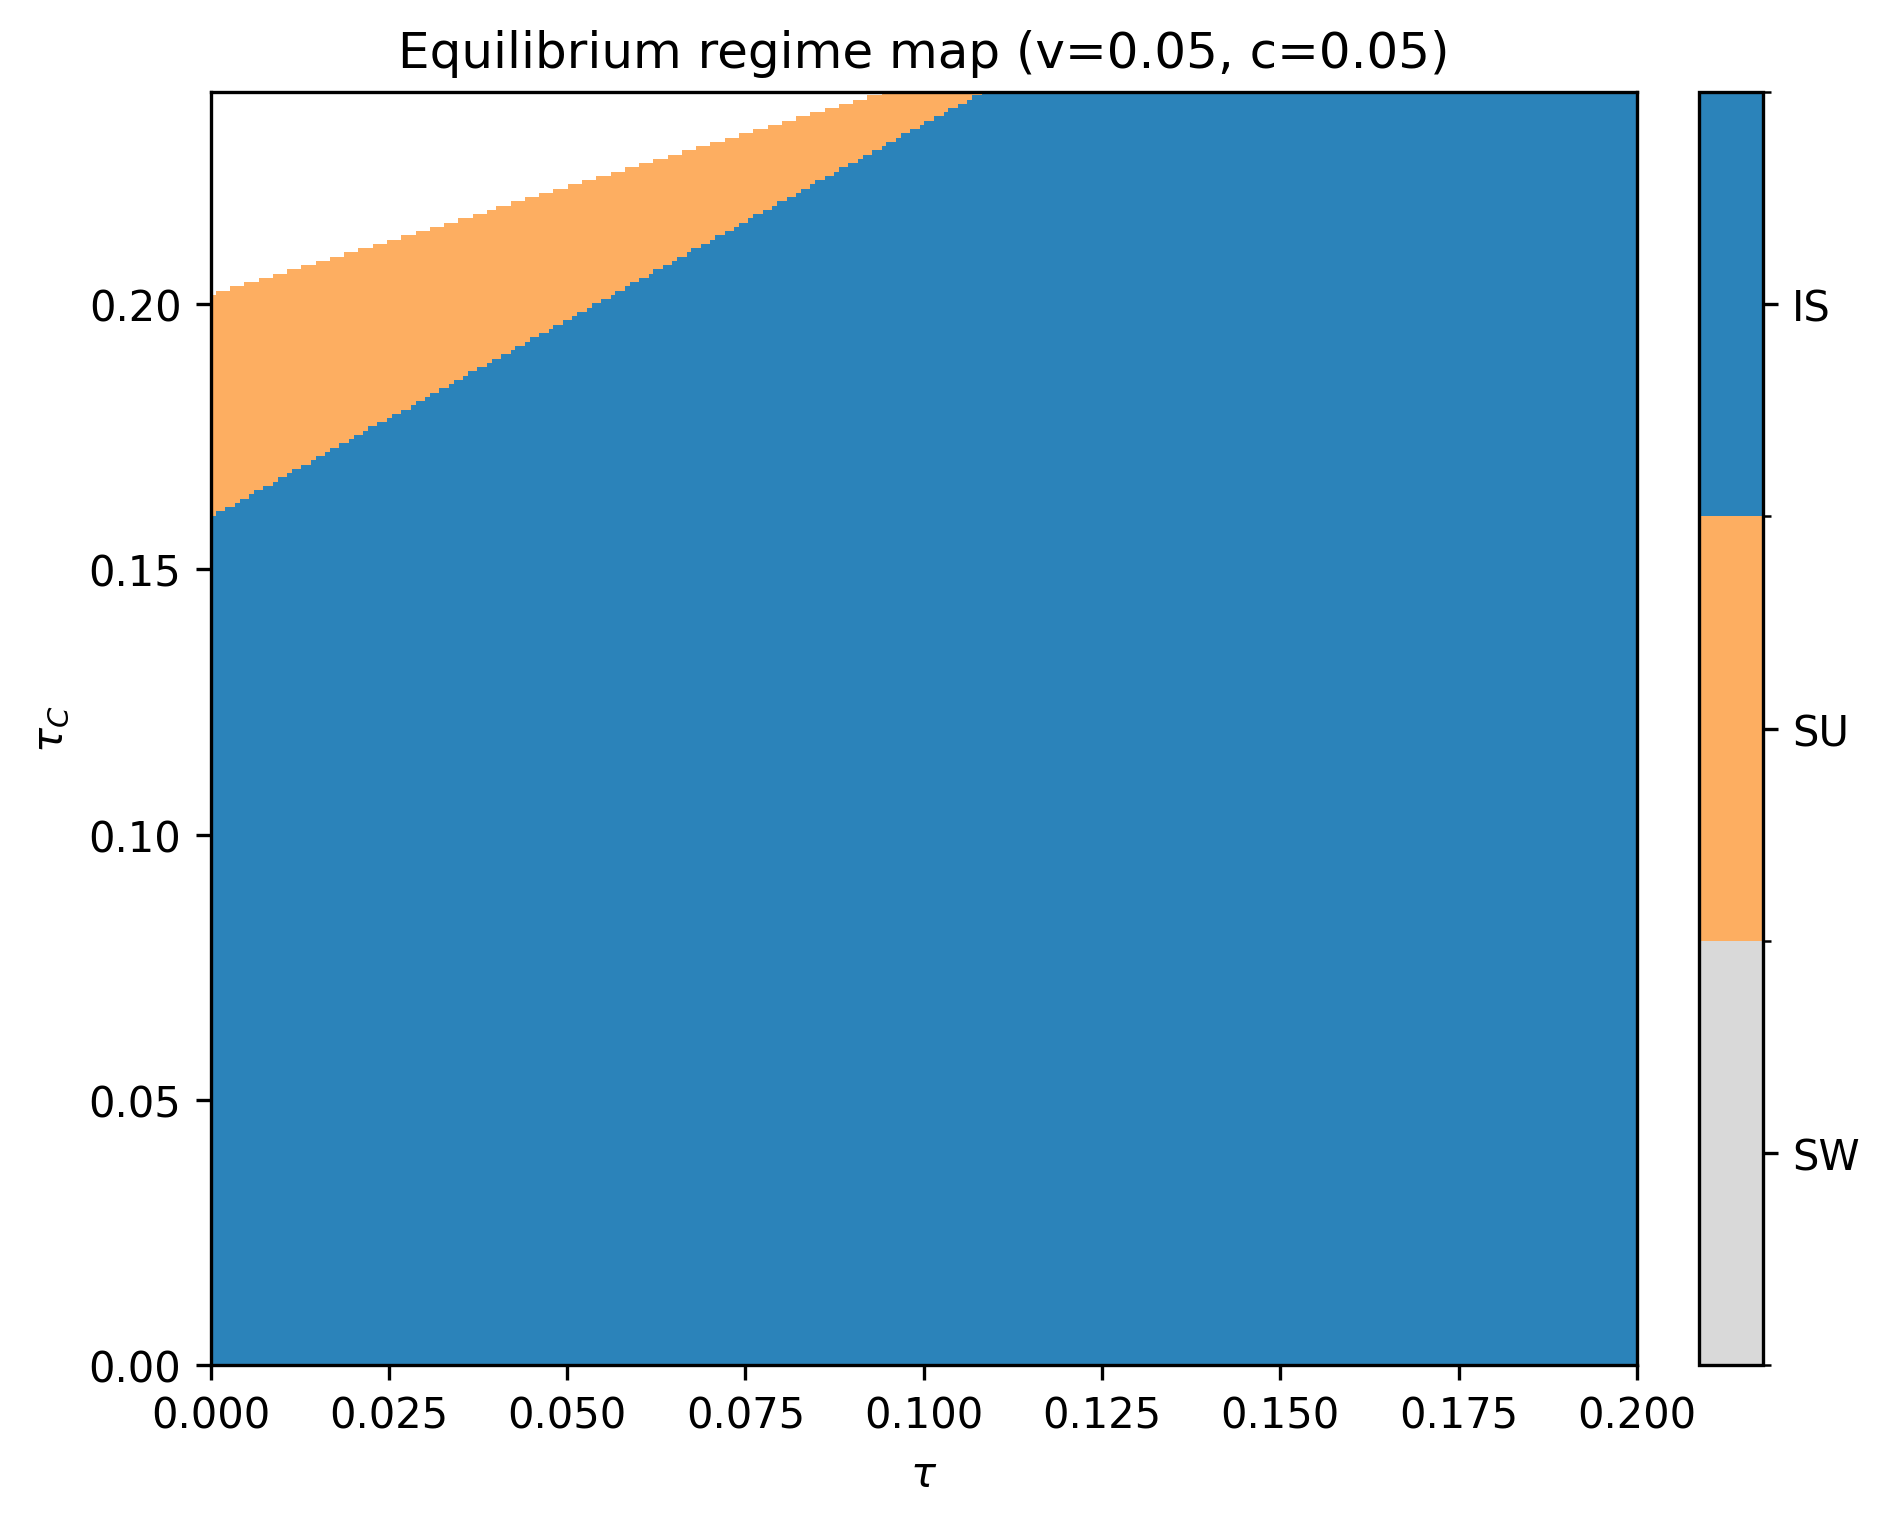
\includegraphics[width=.82\linewidth]{figures/fig2_regime_map.png}
\caption{Equilibrium regime map in $(\tau,\tau_C)$. For fixed $(v,c)$, the figure partitions the $(\tau,\tau_C)$ plane into the regions in which the equilibrium regime characterized by Proposition~\ref{prop:regime_choice_main} is $SW$, $SU$, or $IS$. The map illustrates how outsider-side participation frictions and member-country residual compliance costs jointly determine whether the equilibrium outcome is no harmonization, an exclusionary two-country bloc, or full international standardization.}
\label{fig:regime_map}
\end{figure}

\subsection{World welfare versus equilibrium regime}

The equilibrium characterization in Proposition~\ref{prop:regime_choice_main}
need not coincide with the continuation world-welfare ranking. The next
proposition states the divergence highlighted in the abstract and introduction.

\begin{proposition}[World welfare and equilibrium regime may diverge]
There exists a nonempty subset $\Omega\subset \mathcal P$ such that
\[
\widehat W^{IS}>\max\{\widehat W^{SU},\widehat W^{SW}\},
\]
while the equilibrium regime characterized in
Proposition~\ref{prop:regime_choice_main} is $SU$. Equivalently, for fixed
stage-0 investments, full international standardization can maximize world
welfare without arising in equilibrium.
\label{prop:welfare_gap_main}
\end{proposition}

\begin{proof}
Consider the parameter point
\[
(v,c,\tau,\tau_C)=(0.05,\,0.05,\,0.02,\,0.18).
\]
Using the closed-form continuation-welfare formulas from Appendix~A gives
\[
\widehat W^{SW}\approx 1.24426,\qquad
\widehat W^{SU}\approx 1.54410,\qquad
\widehat W^{IS}\approx 1.67046.
\]
Hence $IS$ strictly maximizes continuation world welfare at this point.
Meanwhile,
\[
\Delta_C^I\approx 0.12788>0,\qquad
\Delta_A^I\approx -0.00076<0,\qquad
\Delta_A^{SU}\approx 0.15189>0.
\]
By Proposition~\ref{prop:regime_choice_main}, the equilibrium regime is
therefore $SU$. Because all inequalities are strict and the closed-form
continuation payoffs are continuous on $\mathcal P$, there exists an open
neighborhood $\Omega$ of this point on which the same inequalities continue to
hold. This proves the claim.
\end{proof}

\noindent\textbf{A one-dimensional characterization of the divergence region.}
The numerical point used in Proposition~\ref{prop:welfare_gap_main} is not
isolated. Fix
\[
(v,c,\tau)=(0.05,0.05,0.02)
\]
and let $\tau_C$ vary. Along this line, the admissibility condition
$1-2c+\tau-3\tau_C>0$ implies
\[
\tau_C<\bar\tau_C^{\,adm}\equiv \frac{1-2c+\tau}{3}=0.306\overline{6}.
\]
Using the closed-form continuation payoffs, the incumbent-acceptance margin
$\Delta_A^I(\tau_C)$ crosses zero at
\[
\tau_C^\dagger \approx 0.1750504.
\]
Moreover, along the same line, both $\Delta_C^I(\tau_C)$ and
$\widehat W^{IS}(\tau_C)-\widehat W^{SU}(\tau_C)$ remain strictly positive
throughout the admissible interval, and $\Delta_A^{SU}(\tau_C)$ is also
strictly positive. Hence for every
\[
\tau_C\in(\tau_C^\dagger,\bar\tau_C^{\,adm}),
\]
the equilibrium regime is $SU$ while continuation world welfare is strictly
higher under $IS$. Thus, Proposition~\ref{prop:welfare_gap_main} is supported
not only by a single benchmark point, but by a nondegenerate interval of
outsider-side compliance costs.

Figure~\ref{fig:divergence_map} shows that the welfare-equilibrium divergence
identified in Proposition~\ref{prop:welfare_gap_main} is not a knife-edge
phenomenon.

\begin{figure}[t]
\centering
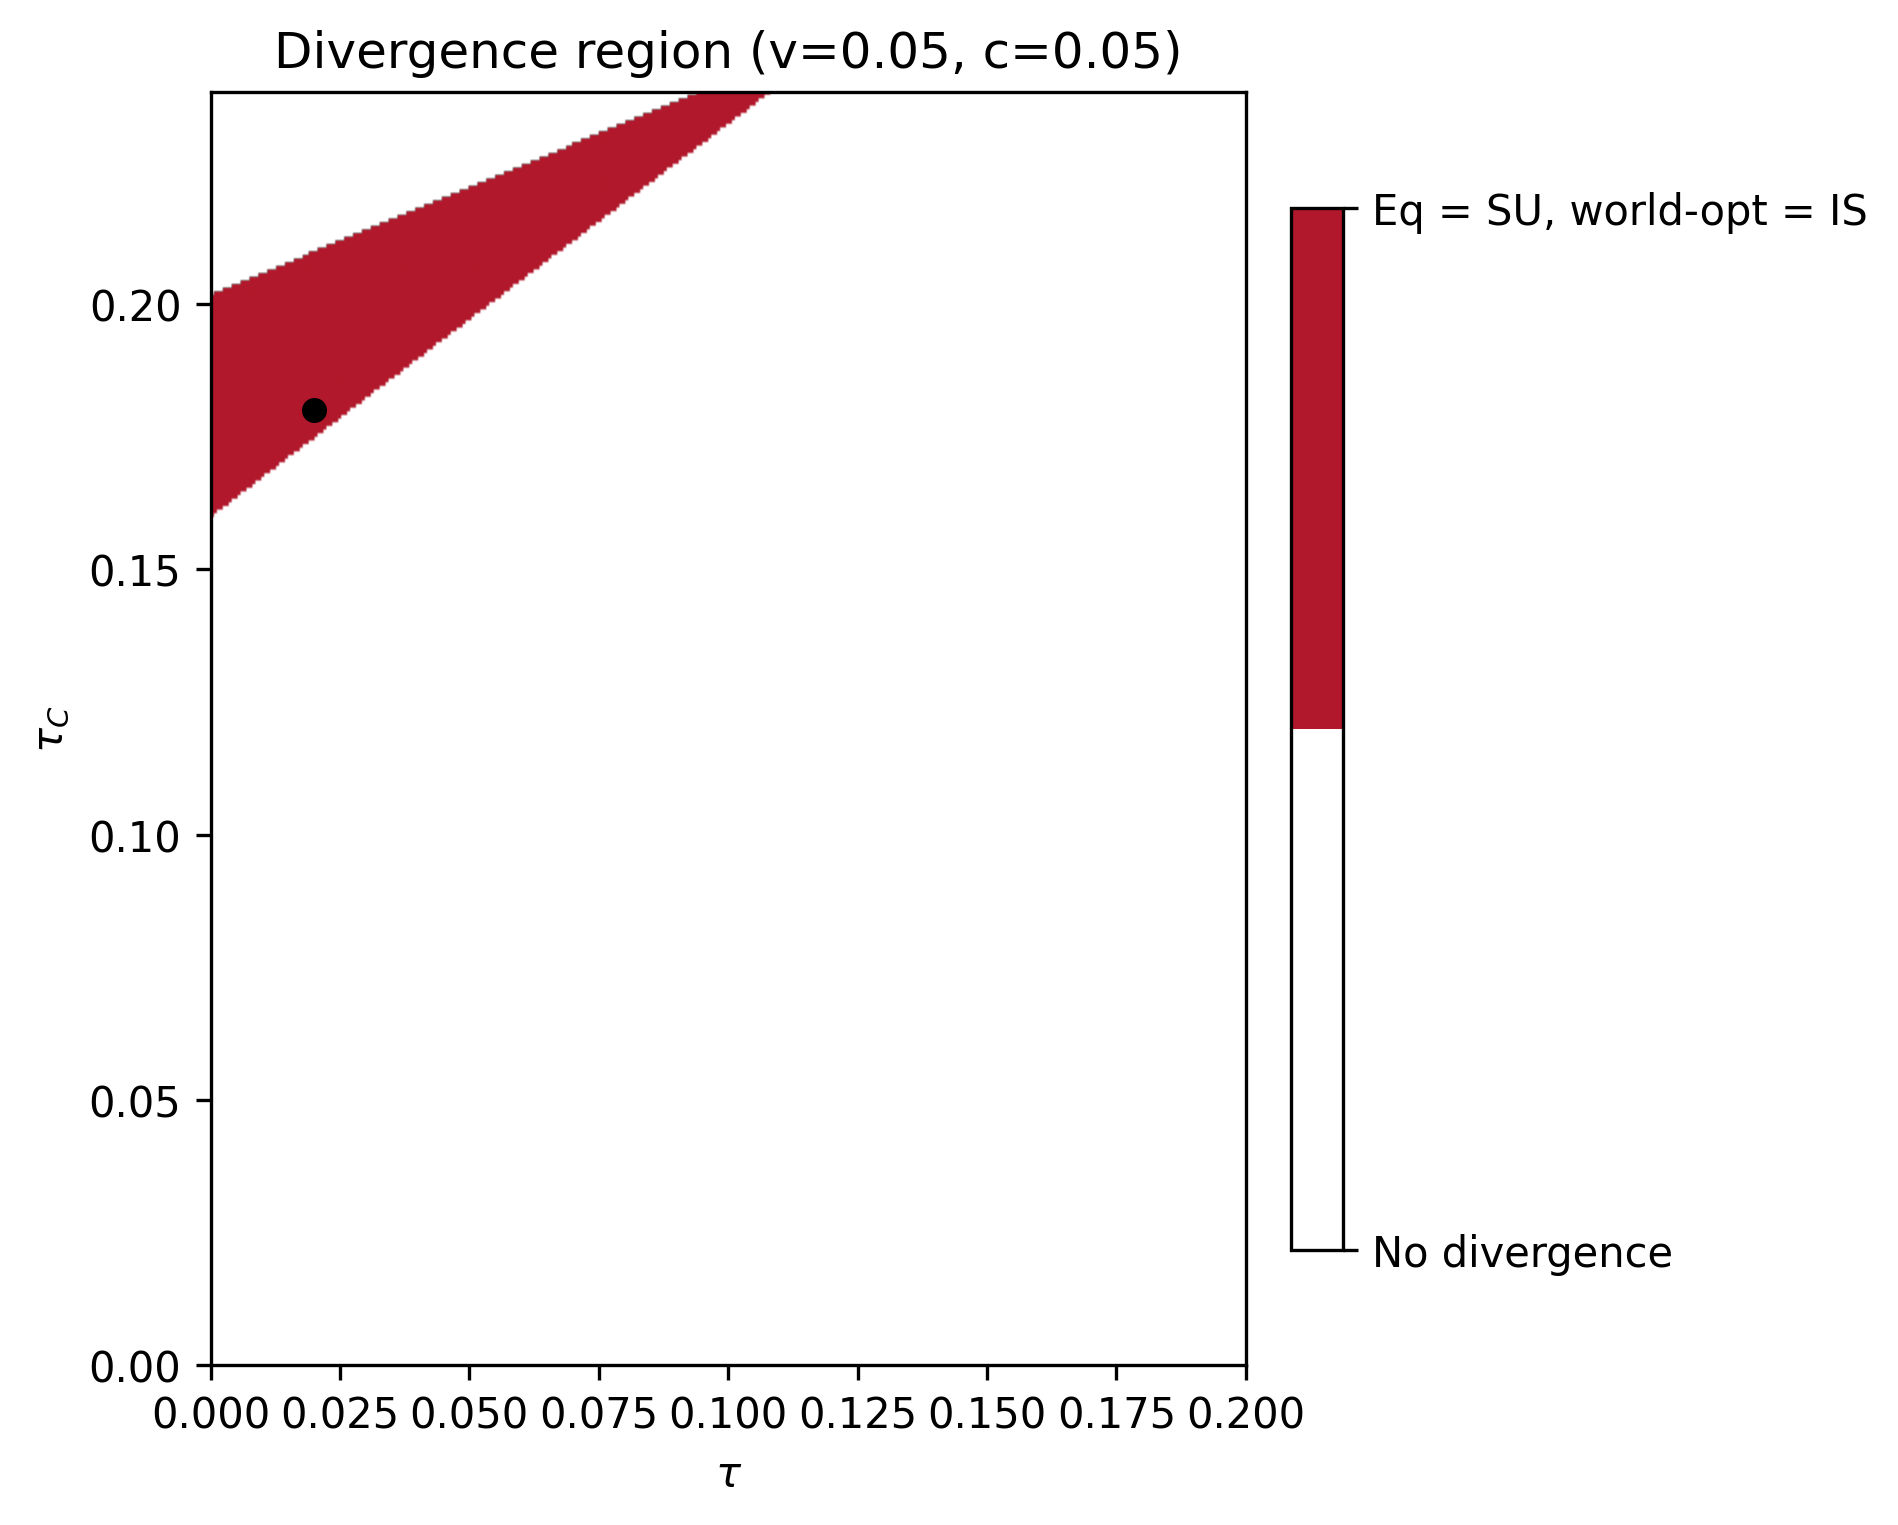
\includegraphics[width=.82\linewidth]{figures/fig3_divergence_map.png}
\caption{Region where the equilibrium regime is $SU$ but the world-optimal regime is $IS$. For fixed $(v,c)$, the shaded region identifies parameter combinations for which incumbent-country incentives sustain an exclusionary two-country bloc even though continuation world welfare is maximized by full international standardization. The benchmark point used in Proposition~\ref{prop:welfare_gap_main}, $(v,c,\tau,\tau_C)=(0.05,0.05,0.02,0.18)$, is marked for reference.}
\label{fig:divergence_map}
\end{figure}

\begin{proposition}[Stronger network effects can stabilize an exclusionary bloc]
There exist parameters $(c,\tau,\tau_C)$ and two network-effect values
$0\le v'<v''<2/7$ such that the equilibrium regime is $IS$ at
$(v',c,\tau,\tau_C)$ but $SU$ at $(v'',c,\tau,\tau_C)$. In particular,
stronger network effects need not favor full harmonization uniformly; they can
instead stabilize an exclusionary two-country standards bloc.
\label{prop:network_bloc_main}
\end{proposition}

\begin{proof}
Consider the common cost profile
\[
(c,\tau,\tau_C)=(0.05,\,0,\,0.15).
\]
At $v'=0.04$, the continuation-welfare differences are
\[
\Delta_A^I\approx 0.00424>0,\qquad
\Delta_C^I\approx 0.11303>0,\qquad
\Delta_A^{IS}\approx 0.12668>0.
\]
By Proposition~\ref{prop:regime_choice_main}, the equilibrium regime is
therefore $IS$.

At $v''=0.055$, the same cost profile yields
\[
\Delta_A^I\approx -0.00026<0,\qquad
\Delta_C^I\approx 0.15025>0,\qquad
\Delta_A^{SU}\approx 0.17261>0.
\]
Hence Proposition~\ref{prop:regime_choice_main} implies that the equilibrium
regime is $SU$. The inequalities are strict at both parameter points, so the
same regime rankings persist on open neighborhoods around them.
\end{proof}

\noindent\textbf{A one-dimensional threshold characterization for Proposition~\ref{prop:network_bloc_main}.}
The mechanism in Proposition~\ref{prop:network_bloc_main} can also be made
more explicit along a fixed cost profile. Set
\[
(c,\tau,\tau_C)=(0.05,0,0.15)
\]
and let $v$ vary. Along this line, the member-country accession margin
$\Delta_A^I(v)$ crosses zero at
\[
v^\dagger \approx 0.0543568.
\]
For $v<v^\dagger$, we have $\Delta_A^I(v)>0$, whereas for $v>v^\dagger$,
$\Delta_A^I(v)<0$. At the same time, $\Delta_C^I(v)>0$,
$\Delta_A^{SU}(v)>0$, and $\widehat W^{IS}(v)-\widehat W^{SU}(v)>0$ continue
to hold throughout the admissible interval in which $SU$ remains interior. In
particular, the relevant admissible upper bound along this line is
\[
\bar v^{\,adm}\approx 0.0756400.
\]
Hence for every
\[
v\in(v^\dagger,\bar v^{\,adm}),
\]
the equilibrium regime is $SU$ even though continuation world welfare remains
strictly higher under $IS$. This yields a one-dimensional threshold
characterization of the network-effect mechanism behind
Proposition~\ref{prop:network_bloc_main}.

\subsection{Interpretation}

Propositions~\ref{prop:regime_choice_main} and \ref{prop:welfare_gap_main}
highlight the role of participation-capacity asymmetry. Even when full
international standardization is technologically feasible, it may fail to arise
for two distinct reasons. First, country $C$ may not find accession attractive
if its residual compliance cost remains too high. Second, even if country $C$
wishes to join, incumbent member countries may reject accession because country
$C$ adds too little to the common network relative to the intensified
competition it creates in member-country markets.

The mechanism behind Proposition~\ref{prop:welfare_gap_main} is straightforward.
When country $C$ has low participation capacity, accession to the common
standard removes the baseline technology-gap cost but still leaves $C$ with a
relatively weak effective competitive position. From the perspective of member
countries $A$ and $B$, accession then delivers only a limited increase in the
common installed base, while it nevertheless introduces additional competition
in member-country markets. As a result, full international standardization can
raise world welfare and still fail the incumbent members' private acceptance
test.

The comparative statics in Appendix~B help sharpen this logic. On the verified
compact domain used in Section~5, both $\Delta_A^I$ and $\Delta_C^I$ decline as
$\tau_C$ rises. Intuitively, a larger outsider-side compliance burden weakens
the outsider's effective market participation even after formal accession. Yet
$\Delta_C^I$ may remain positive longer than $\Delta_A^I$, because country $C$
still values the removal of the baseline technology-gap cost under $IS$, while
member governments internalize the additional competition in their own markets.

Proposition~\ref{prop:network_bloc_main} shows that the network parameter $v$
does not operate monotonically in favor of full harmonization. Stronger network
effects magnify the installed-base gain from common recognition, but they also
raise the strategic value of preserving an incumbent bloc when outsider
participation remains weak. Accordingly, an exclusionary two-country standards
bloc may persist not only because incumbent countries strategically prefer
exclusion, but also because the outsider's participation capacity is too weak
for full harmonization to be privately attractive.


% =================================================
% Section 5
% =================================================
\section{Capacity Investment and Transfer Policy}

This section returns to stage 0 and studies how capacity-building policy
affects the equilibrium standardization regime. The key idea is simple:
capacity investment lowers residual compliance costs, and thereby changes the
incentives to form a two-country bloc, to request accession, and to accept
accession.

The results in this section are intentionally more conditional than those in
Sections~3--4. From this point onward, we work with the monotonicity structure
discussed in Appendix~B to ensure that the relevant regime-comparison
functions cross zero in a well-behaved way on an explicit compact parameter
set. Accordingly, the results of Section~5 are local-to-domain comparative
statics established on the verified compact set $\mathcal D'$ reported in
Appendix~B, rather than unrestricted global statements over the entire
admissible set $\mathcal P$.
In particular, the threshold objects used below are established on the
verified compact domain $\mathcal D'$ reported in Appendix~B and rely on two
ingredients: (i) the monotonicity inequalities, which are numerically verified
on $\mathcal D'$, and (ii) the endpoint crossing conditions stated in
Appendix~B.

\subsection{Stage-0 capacity investment}

Recall that participation capacity is given by
\[
\theta_k=\bar\theta_k+I_k,
\qquad
I_k\in[0,1-\bar\theta_k],
\]
and that the residual compliance cost is
\[
\tau_k=\mu(1-\theta_k), \qquad \mu>0.
\]
It is convenient to rewrite this as
\begin{equation}
\tau_k=\bar\tau_k-\mu I_k,
\qquad
\bar\tau_k\equiv \mu(1-\bar\theta_k).
\label{eq:tau_from_x}
\end{equation}

To preserve the symmetry structure of Sections~3 and 4, we focus on symmetric
stage-0 investments by the two high-capacity countries:
\[
I_A=I_B\equiv I_H,
\qquad
\bar\tau_A=\bar\tau_B\equiv \bar\tau.
\]
Hence the post-investment residual costs are
\begin{equation}
\tau=\bar\tau-\mu I_H,
\qquad
\tau_C=\bar\tau_C-\mu I_C.
\label{eq:tau_tauC_from_x}
\end{equation}

Let
\[
R(\tau,\tau_C)\in\{SW,SU,IS\}
\]
denote the equilibrium regime characterized in
Proposition~\ref{prop:regime_choice_main}. At stage 0, government
$H\in\{A,B\}$ and government $C$ choose investments anticipating this regime
map. Their full payoffs are
\begin{align}
\Omega_H(I_H,I_C)
&=
\widehat W_A^{R(\tau,\tau_C)}(\tau,\tau_C)
-\frac{\eta}{2}I_H^2, \label{eq:OmegaH}\\
\Omega_C(I_H,I_C)
&=
\widehat W_C^{R(\tau,\tau_C)}(\tau,\tau_C)
-\frac{\eta}{2}I_C^2, \label{eq:OmegaC}
\end{align}
where $\tau$ and $\tau_C$ are given by \eqref{eq:tau_tauC_from_x}.

Because the regime map is piecewise constant, the stage-0 problem is piecewise
smooth. Inside any region in which the continuation regime is fixed at some
$r\in\{SW,SU,IS\}$, the local investment problem is standard.

\noindent\textbf{Scope of the stage-0 analysis.}
We do not attempt a full global characterization of the simultaneous stage-0
Nash equilibrium across all regime boundaries. The purpose of Section~5 is
narrower: to identify the threshold directions through which capacity
investment shifts regime selection, and to compare the qualitative policy
effects of outsider-side and member-side capacity adjustments on the verified
compact domain reported in Appendix~B.

\begin{lemma}[Local investment condition under a fixed regime]
\label{lem:local_investment_condition}
Fix a regime $r\in\{SW,SU,IS\}$ and suppose that $(\tau,\tau_C)$ lies in the
interior of the region in which $R(\tau,\tau_C)=r$. Then any interior local
optimum of the stage-0 investment problem satisfies
\begin{align}
\eta I_H &= -\mu \frac{\partial \widehat W_A^r(\tau,\tau_C)}{\partial \tau},
\label{eq:FOC_IH}\\
\eta I_C &= -\mu \frac{\partial \widehat W_C^r(\tau,\tau_C)}{\partial \tau_C}.
\label{eq:FOC_IC}
\end{align}
\end{lemma}

\begin{proof}
From \eqref{eq:tau_tauC_from_x}, we have
\[
\frac{\partial \tau}{\partial I_H}=-\mu,
\qquad
\frac{\partial \tau_C}{\partial I_C}=-\mu.
\]
Within a fixed regime $r$, \eqref{eq:OmegaH} and \eqref{eq:OmegaC} are
differentiable, so the first-order conditions are
\[
\frac{\partial \Omega_H}{\partial I_H}
=
\frac{\partial \widehat W_A^r}{\partial \tau}\frac{\partial \tau}{\partial I_H}
-\eta I_H
=
-\mu\frac{\partial \widehat W_A^r}{\partial \tau}
-\eta I_H
=0,
\]
and
\[
\frac{\partial \Omega_C}{\partial I_C}
=
\frac{\partial \widehat W_C^r}{\partial \tau_C}\frac{\partial \tau_C}{\partial I_C}
-\eta I_C
=
-\mu\frac{\partial \widehat W_C^r}{\partial \tau_C}
-\eta I_C
=0,
\]
which gives \eqref{eq:FOC_IH}--\eqref{eq:FOC_IC}.
\end{proof}

Lemma~\ref{lem:local_investment_condition} has an immediate interpretation.
Investment is chosen up to the point where its marginal cost equals the
marginal gain from reducing the relevant residual compliance cost. However,
because the equilibrium regime itself depends on $(\tau,\tau_C)$, governments
may also invest strategically in order to cross a regime boundary.

\subsection{Investment thresholds and regime switching}

The regime conditions in Proposition~\ref{prop:regime_choice_main} can be
translated directly into investment thresholds. To state this cleanly, assume
that the welfare differences in Section~4 satisfy the following monotonicity
property on the relevant domain:
\begin{equation}
\frac{\partial \Delta_A^I}{\partial \tau_C}<0,
\qquad
\frac{\partial \Delta_C^I}{\partial \tau_C}<0,
\qquad
\frac{\partial \Delta_A^{SU}}{\partial \tau}<0,
\qquad
\frac{\partial \Delta_A^{IS}}{\partial \tau}<0.
\label{eq:monotonicity}
\end{equation}

Condition \eqref{eq:monotonicity} says that a higher outsider residual cost
makes accession less attractive both to the outsider and to incumbent members,
while a higher member-country residual cost makes bilateral or full
harmonization less attractive relative to $SW$. Appendix~B verifies these
signs numerically on the broader compact domain
\[
\mathcal D'
=
\left\{
\begin{aligned}
(v,c,\tau,\tau_C):\quad &0 \le v \le 0.055,\\
&0.03 \le c \le 0.06,\\
&0 \le \tau \le 0.04,\\
&0 \le \tau_C \le 0.18
\end{aligned}
\right\}
\subset \mathcal P,
\]
which contains the paper's benchmark numerical examples and a wider range of
baseline trade-cost values.

Under \eqref{eq:monotonicity}, define the accession thresholds
$\tau_C^A(\tau)$ and $\tau_C^C(\tau)$ implicitly by
\begin{align}
\Delta_A^I(\tau,\tau_C^A(\tau)) &= 0, \label{eq:tauCA_def}\\
\Delta_C^I(\tau,\tau_C^C(\tau)) &= 0, \label{eq:tauCC_def}
\end{align}
whenever such roots exist, and define the effective accession threshold
\begin{equation}
\tau_C^{I}(\tau)\equiv \min\{\tau_C^A(\tau),\tau_C^C(\tau)\}.
\label{eq:tauCI_def}
\end{equation}
Likewise, define the member-side formation thresholds $\tau^{SU}(\tau_C)$ and
$\tau^{IS}(\tau_C)$ implicitly by
\begin{align}
\Delta_A^{SU}(\tau^{SU}(\tau_C),\tau_C) &= 0, \label{eq:tauSU_def}\\
\Delta_A^{IS}(\tau^{IS}(\tau_C),\tau_C) &= 0. \label{eq:tauIS_def}
\end{align}

These cost thresholds induce corresponding investment thresholds. In
particular, using \eqref{eq:tau_tauC_from_x}, the minimum outsider investment
required to make accession feasible is
\begin{equation}
I_C^{I}(I_H)
\equiv
\max\left\{
0,\,
\frac{\bar\tau_C-\tau_C^{I}(\bar\tau-\mu I_H)}{\mu}
\right\}.
\label{eq:xC_threshold}
\end{equation}

\begin{proposition}[Capacity thresholds and the equilibrium regime]
Suppose \eqref{eq:monotonicity} holds and the threshold functions defined in
\eqref{eq:tauCA_def}--\eqref{eq:tauIS_def} exist.

\begin{enumerate}
    \item For any given member-country investment $I_H$, accession is feasible
    if and only if
    \[
    I_C \ge I_C^I(I_H).
    \]

    \item If accession is feasible and
    \[
    \Delta_A^{IS}(\bar\tau-\mu I_H,\bar\tau_C-\mu I_C)\ge 0,
    \]
    then the equilibrium regime is $IS$.

    \item If accession is not feasible and
    \[
    \Delta_A^{SU}(\bar\tau-\mu I_H,\bar\tau_C-\mu I_C)\ge 0,
    \]
    then the equilibrium regime is $SU$.

    \item Otherwise, the equilibrium regime is $SW$.
\end{enumerate}
\label{prop:investment_thresholds}
\end{proposition}

\begin{proof}
By Proposition~\ref{prop:regime_choice_main}, $IS$ requires $\Delta_A^I\ge 0$,
$\Delta_C^I\ge 0$, and $\Delta_A^{IS}\ge 0$. Under
\eqref{eq:monotonicity}, the first two inequalities are equivalent to
\[
\tau_C\le \tau_C^A(\tau)
\quad\text{and}\quad
\tau_C\le \tau_C^C(\tau),
\]
which together are equivalent to
\[
\tau_C\le \tau_C^I(\tau).
\]
Using \eqref{eq:tau_tauC_from_x}, this condition becomes
\[
\bar\tau_C-\mu I_C \le \tau_C^{I}(\bar\tau-\mu I_H),
\]
or equivalently
\[
I_C \ge
\frac{\bar\tau_C-\tau_C^{I}(\bar\tau-\mu I_H)}{\mu}.
\]
Imposing the non-negativity constraint on investment yields
\eqref{eq:xC_threshold}. Parts (2)--(4) then follow immediately from
Proposition~\ref{prop:regime_choice_main}.
\end{proof}

Figure~\ref{fig:investment_map} translates the threshold structure of
Proposition~\ref{prop:investment_thresholds} into policy space and shows how
outsider-side and member-side capacity investment move the economy across
regime boundaries.

\begin{figure}[t]
\centering
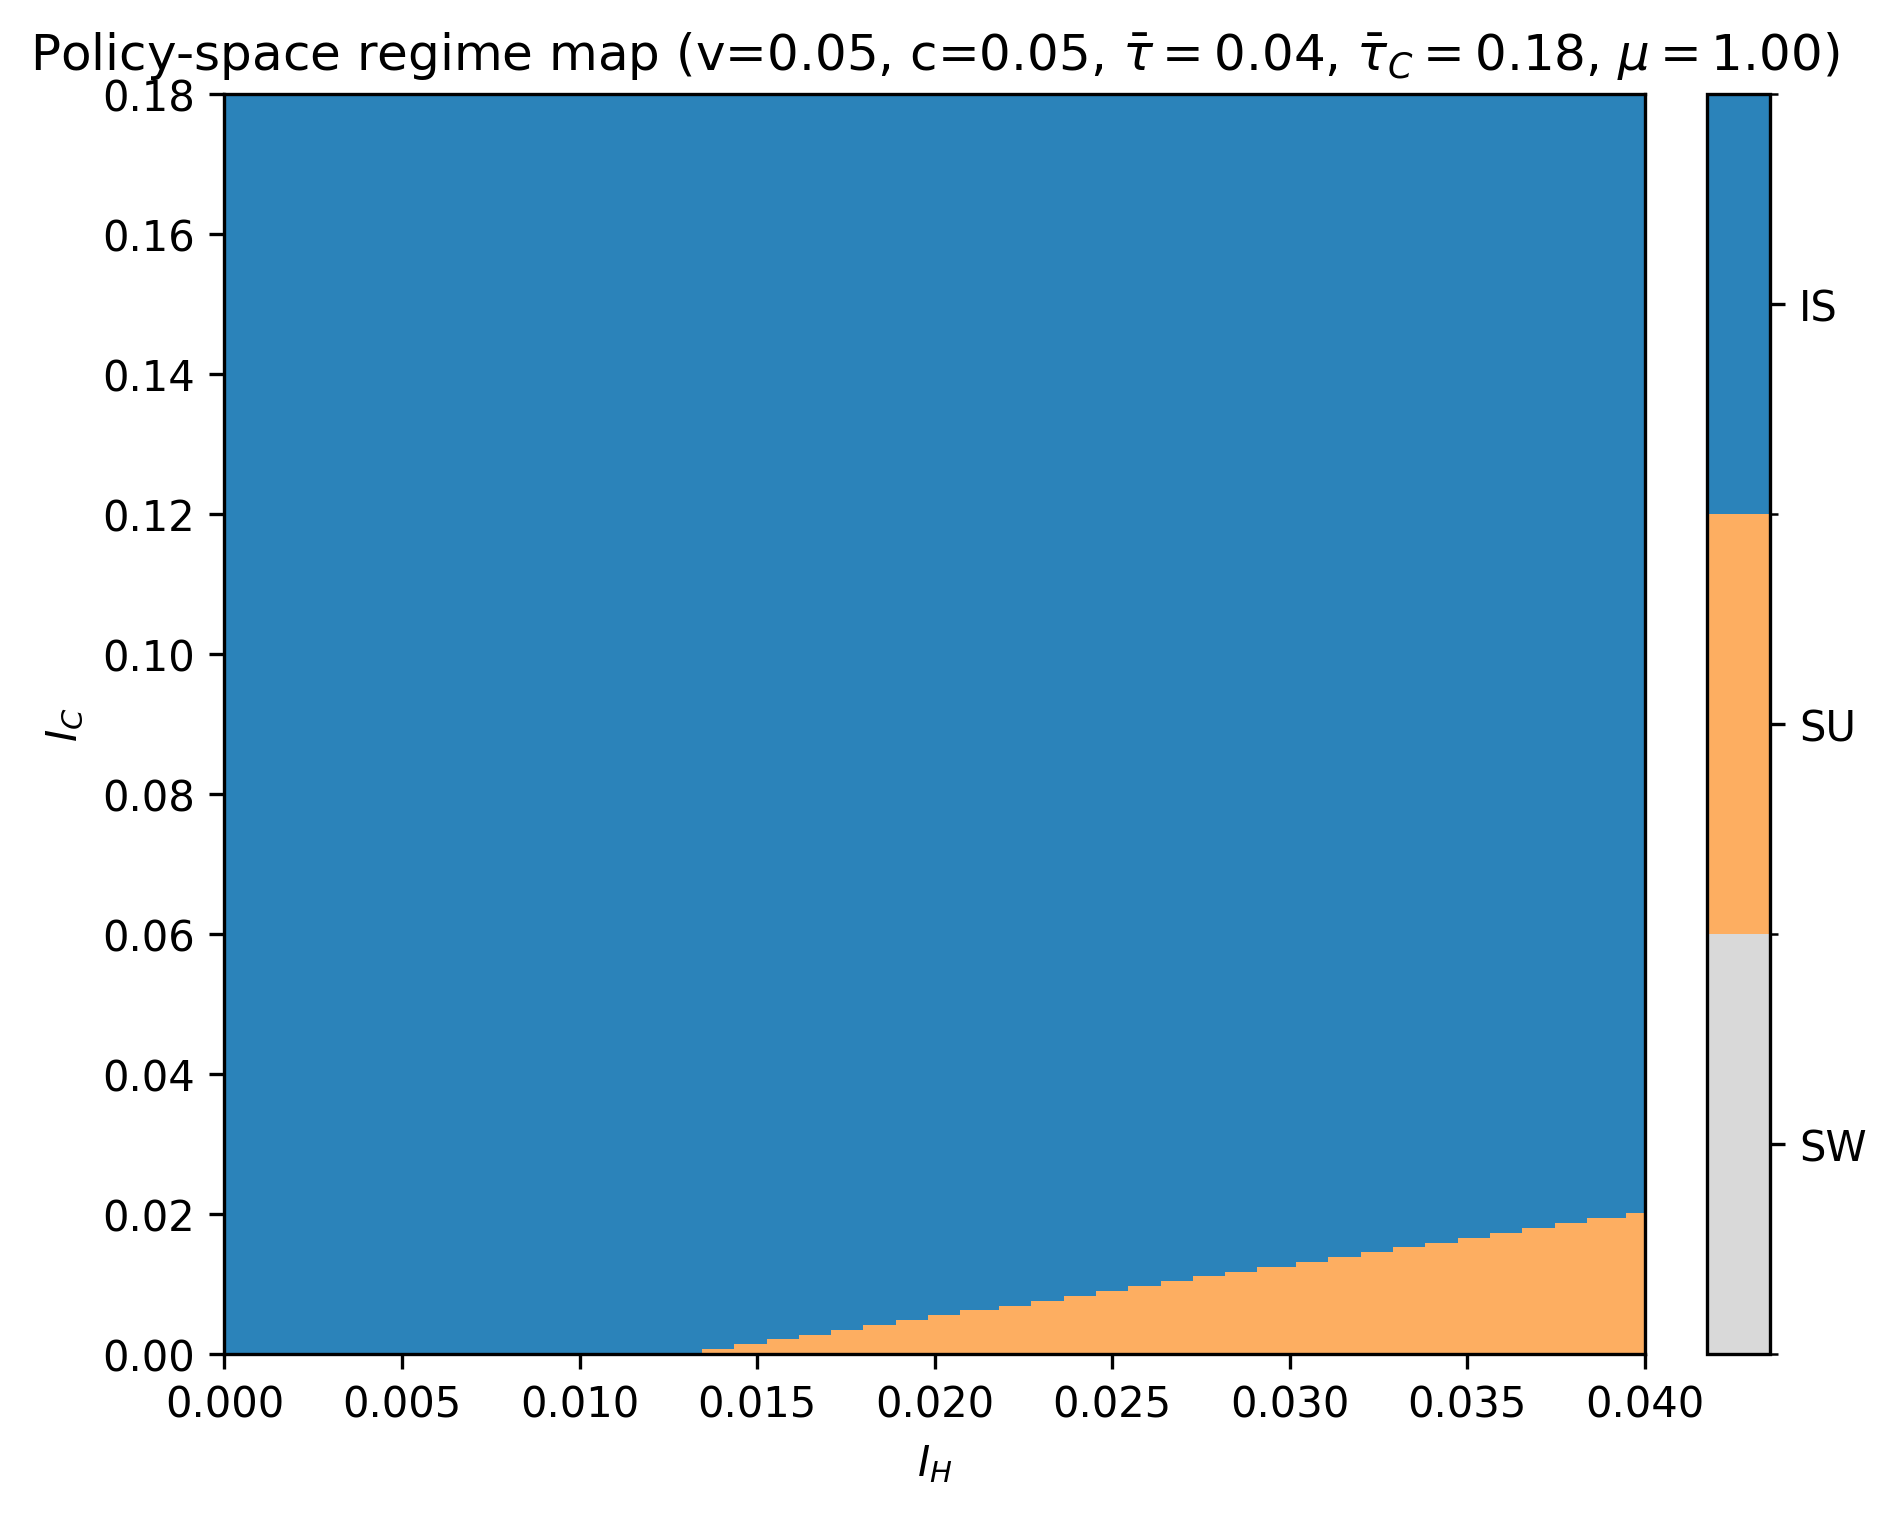
\includegraphics[width=.82\linewidth]{figures/fig4_investment_map.png}
\caption{Policy-space regime map in $(I_H,I_C)$. For fixed primitive parameters $(v,c,\bar{\tau},\bar{\tau}_C,\mu)$, the figure maps the equilibrium regime into the investment space of member-country and outsider-country capacity building. The boundary associated with outsider-side investment captures the effective accession constraint, while the member-side boundary captures the bloc-formation versus harmonization margin emphasized in Proposition~\ref{prop:investment_thresholds}.}
\label{fig:investment_map}
\end{figure}

Proposition~\ref{prop:investment_thresholds} yields a sharp interpretation.
Outsider-side capacity investment mainly relaxes the accession constraint,
while member-side capacity investment mainly relaxes the bloc-formation
constraint. In that sense, the two types of investment operate on different
margins of the regime-selection game.

\subsection{Conditional transfer policy}

Capacity building need not rely exclusively on domestic investment by country
$C$. An international organization, a regional agreement, or the incumbent
member countries may provide technical assistance, certification support, or
conformity-assessment aid. To capture this possibility, suppose that a
conditional transfer $s\ge 0$ can be offered to country $C$.

The transfer is \emph{conditional}: it is implemented only if $IS$ is
realized. Thus, under $IS$, the outsider's effective residual compliance cost
becomes
\begin{equation}
\tau_C^{\,IS}(s)=\tau_C-s,
\qquad
0\le s\le \tau_C,
\label{eq:tauC_transfer}
\end{equation}
whereas payoffs under $SU$ and $SW$ remain unchanged. Let the resource cost of
the transfer be
\begin{equation}
G(s)=\frac{\kappa}{2}s^2,
\qquad \kappa>0.
\label{eq:Gs}
\end{equation}

The transfer $s$ should be interpreted as a reduced-form policy instrument
representing accession-contingent capacity assistance, such as testing support,
certification infrastructure, or implementation aid. The function $G(s)$
captures the real resource cost of providing such support, including
administrative and financing costs. Thus, the policy experiment is not a pure
redistribution exercise, but a stylized way to model costly external support
targeted at the participation bottleneck.

The transfer instrument $s$ is modeled as a planner policy rather than as a
decentralized side payment chosen directly by incumbent member governments. Its
purpose is to capture costly accession-contingent capacity assistance without
embedding a separate bargaining game over who finances the transfer. Modeling
decentralized funding incentives for the transfer is an interesting extension,
but it is outside the scope of the present paper.

Recall the continuation world-welfare measure from
\eqref{eq:world_continuation}:
\[
\widehat W^r(\tau,\tau_C)\equiv 2\widehat W_A^r(\tau,\tau_C)+\widehat W_C^r(\tau,\tau_C).
\]

Because the transfer operates only when $IS$ is implemented, any transfer
level below the accession-enabling threshold is outcome-equivalent to no
transfer at all. Accordingly, the central object is the minimum transfer that
makes accession feasible:
\begin{equation}
s^{acc}(\tau,\tau_C)
\equiv
\max\{0,\tau_C-\tau_C^I(\tau)\}.
\label{eq:sacc}
\end{equation}

The international planner's problem is therefore
\begin{equation}
\max_{s\ge 0}
\left\{
\widehat W^{IS}(\tau,\tau_C-s)-G(s)
\right\}
\quad
\text{subject to }
s\ge s^{acc}(\tau,\tau_C),
\label{eq:planner_transfer}
\end{equation}
with the outside option given by the equilibrium continuation welfare under no
transfer.

\begin{proposition}[Optimal conditional transfer]
Suppose \eqref{eq:monotonicity} holds and $G$ is strictly convex with
$G(0)=0$.

\begin{enumerate}
    \item Any welfare-improving conditional transfer is either zero or at
    least $s^{acc}(\tau,\tau_C)$.

    \item If the optimal transfer is interior and positive, it satisfies
    \begin{equation}
    -\frac{\partial \widehat W^{IS}(\tau,\tau_C-s)}{\partial \tau_C}
    =
    G'(s).
    \label{eq:transfer_FOC}
    \end{equation}

    \item If
    \begin{equation}
    \widehat W^{IS}(\tau,\tau_C-s^{acc})-G(s^{acc})
    \ge
    \max\{\widehat W^{SU}(\tau,\tau_C),\,\widehat W^{SW}(\tau,\tau_C)\},
    \label{eq:transfer_gain}
    \end{equation}
    then there exists an optimal transfer that induces $IS$. Otherwise, the
    planner sets $s=0$ and the no-transfer regime persists.
\end{enumerate}
\label{prop:transfer}
\end{proposition}

\begin{proof}
Part (1) follows directly from the conditionality of the transfer. If
$0<s<s^{acc}$, then accession remains infeasible by \eqref{eq:sacc}, so the
transfer is never implemented. Hence such a transfer is equivalent to $s=0$.

For part (2), conditional on choosing a transfer that induces $IS$, the
planner solves the unconstrained problem
\[
\max_{s\ge s^{acc}}
\left\{
\widehat W^{IS}(\tau,\tau_C-s)-G(s)
\right\}.
\]
The derivative with respect to $s$ is
\[
-\frac{\partial \widehat W^{IS}(\tau,\tau_C-s)}{\partial \tau_C}-G'(s).
\]
Setting this equal to zero gives \eqref{eq:transfer_FOC}.

For part (3), if \eqref{eq:transfer_gain} holds, then the planner weakly
prefers inducing $IS$ with the minimum accession-enabling transfer to any
no-transfer continuation. By strict convexity of $G$, an optimal transfer
exists. If \eqref{eq:transfer_gain} fails, then every transfer that induces
$IS$ yields continuation welfare weakly below the best no-transfer outcome, so
the planner optimally sets $s=0$.
\end{proof}

\subsection{Policy implication}

Proposition~\ref{prop:transfer} clarifies the economic role of transfer policy,
conditional on the verified monotonicity structure imposed above. Standards
fragmentation may persist even when full harmonization is technologically
feasible, because country $C$'s participation capacity is too weak for
accession to be privately attractive. In that case, conditional capacity aid
can restore the missing participation margin directly, rather than trying to
alter the equilibrium indirectly through protectionist standard policies.

The model therefore suggests a conditional policy ranking on the verified
compact domain studied here. When exclusion is driven primarily by
participation-capacity asymmetry, targeted capacity-building measures---such as
technical assistance, testing infrastructure, certification support, or
mutual-recognition implementation aid---are more effective, in the present
framework, at restoring the accession margin than policies that merely
preserve fragmented national standards. In the present framework, the latter
should be interpreted as
policies that maintain the outsider's effective separation from the common
recognition area, rather than as instruments that directly relax the
compliance bottleneck itself.

Finally, the analysis also suggests a reason why decentralized investment may
fall short of what would be desirable from a broader international
perspective. This point should be read as an economic implication of the model
rather than as a separate global theorem. Each government chooses investment
by comparing its own marginal gain with its own marginal cost, as in
\eqref{eq:FOC_IH}--\eqref{eq:FOC_IC}. But accession to a common standard can
create cross-country benefits through market expansion and a larger installed
base, and those gains are not fully internalized by any single government
when investment is chosen non-cooperatively. In that sense, the decentralized
investment benchmark may be too low relative to a coordinated benchmark that
values the full international surplus created by effective accession.
Conditional transfer policy is one possible instrument for narrowing that gap.


% =================================================
% Section 6
% =================================================
\section{Conclusion}

This paper has studied international standardization in a three-country model with network externalities, coalition formation, and asymmetric participation capacity. The key distinction developed here is between \emph{formal accession} to a common standard and \emph{effective participation} in that standard. Mutual recognition may eliminate the baseline technology-gap cost within a recognition area, yet countries can still differ in their ability to comply with, test, certify, and implement the common standard. Once that distinction is introduced, the equilibrium logic of international standardization changes in economically meaningful ways.

The analysis delivers three main conclusions. First, full international standardization may be globally efficient without arising in equilibrium. A low-capacity outsider may add too little to the common installed base, relative to the additional competitive pressure its accession creates in incumbent-member markets, for full harmonization to be privately attractive to the member governments. Second, stronger network effects do not necessarily favor full harmonization uniformly. On a verified parameter region with pronounced participation-capacity asymmetry, stronger network effects can instead stabilize an exclusionary two-country standards bloc. Third, once participation capacity is endogenized, capacity-building investment and conditional transfer policy can, on the verified compact domain used in Section~5, restore the missing accession margin more effectively than policies that merely preserve fragmented national standards.

These results contribute to the literature in a simple but useful way. Relative to the classic compatibility literature, the paper shows that compatibility and participation should not be treated as synonymous. Relative to the international standardization literature, it identifies a mechanism through which inefficient exclusion can persist even when mutual recognition is technologically feasible. Relative to recent empirical work on standards, trade, and innovation, it offers a tractable framework for thinking about how asymmetries in compliance and implementation capacity may shape the formation and persistence of standards blocs.

The policy message is equally direct, but it should be read with the qualification emphasized in Section~5. If fragmentation persists because weaker countries cannot participate effectively in a harmonized regime, then the relevant intervention is not limited to the legal act of recognition itself. What matters is whether participation capacity can be raised through investment in testing, certification, conformity assessment, and related implementation capabilities. In the model, such policies relax the actual bottleneck in the regime-selection game, whereas policies that merely preserve fragmented national standards leave that bottleneck in place. This suggests that capacity-oriented assistance may be a more effective response to inefficient fragmentation than policies centered solely on preserving domestic standard autonomy.
This policy conclusion should be interpreted in the same qualified sense as
the threshold analysis in Section~5: it is established on the verified compact
domain reported in Appendix~B and under the corresponding crossing
conditions, rather than as an unrestricted claim over all admissible parameter
values.

The paper also points to several natural extensions. One would be to endogenize coalition formation more fully, allowing for simultaneous three-country negotiation or asymmetric bilateral bargaining involving country $C$ rather than the benchmark accession game studied here. Another would be to allow firms to choose not only quantities but also whether to adopt foreign or international standards strategically. A third would be to introduce partial interoperability, rather than the sharp distinction between exclusion and full membership used here. A fourth extension would be to connect the theoretical threshold conditions more directly to empirical measures of participation capacity, for example using data on standardization activity, certification infrastructure, or international standard adoption. Such extensions would help clarify how formal standardization institutions interact with implementation capacity in practice.

More broadly, the paper suggests that the economics of international standardization should pay greater attention to the difference between joining a rule system and being able to operate effectively within it. In markets shaped by network effects and compatibility decisions, that distinction can determine whether harmonization becomes genuinely inclusive or remains organized around exclusionary blocs.


% =================================================
% Appendices
% =================================================
\appendix

\appendix
\section{Explicit Continuation-Welfare Formulas and Proof Skeleton}

\subsection{Preliminaries}

Throughout this appendix, $\mathcal P$ denotes the admissible parameter set
defined in Section~3. On $\mathcal P$, all denominators in the
continuation-welfare level formulas reported below are strictly positive.
Appendix~B studies derivatives of welfare differences; those expressions
contain an additional factor $(v-1)$ after simplification, so their
denominators are strictly negative on $\mathcal P$. The two sign statements
therefore refer to different objects.

A useful implication of the exact stage-4 first-order conditions is that profits can be written in a compact form:
\begin{align}
\pi_A^{SW} &= (x^{SW})^2+(y^{SW})^2+(w^{SW})^2, &
\pi_C^{SW} &= 2(z^{SW})^2+(t^{SW})^2, \label{eq:profit_id_sw}\\
\pi_A^{SU} &= (1-v)\Big[(x^{SU})^2+(y^{SU})^2+(w^{SU})^2\Big], &
\pi_C^{SU} &= 2(z^{SU})^2+(t^{SU})^2, \label{eq:profit_id_su}\\
\pi_A^{IS} &= (1-v)\Big[(x^{IS})^2+(y^{IS})^2+(w^{IS})^2\Big], &
\pi_C^{IS} &= (1-v)\Big[2(z^{IS})^2+(t^{IS})^2\Big]. \label{eq:profit_id_is}
\end{align}
Together with $CS_k^r=(Q_k^r)^2/2$, these identities yield compact continuation-welfare formulas.

\subsection{Continuation welfare under \texorpdfstring{$SW$}{SW}}

Under $SW$,
\begin{align}
x^{SW} &= \frac{1+2c+\tau+\tau_C}{4}, &
y^{SW} &= \frac{1-2c-3\tau+\tau_C}{4}, \notag\\
z^{SW} &= \frac{1-2c+\tau-3\tau_C}{4}, &
w^{SW} &= \frac{1-2c-2\tau}{4}, \notag\\
t^{SW} &= \frac{1+2c+2\tau}{4}, \label{eq:sw_outputs_appendix}
\end{align}
and aggregate quantities are
\begin{align}
Q_A^{SW} &= x^{SW}+y^{SW}+z^{SW}
= \frac{3-2c-\tau-\tau_C}{4}, \label{eq:QA_sw_appendix}\\
Q_C^{SW} &= 2w^{SW}+t^{SW}
= \frac{3-2c-2\tau}{4}. \label{eq:QC_sw_appendix}
\end{align}

Hence
\begin{align}
\widehat W_A^{SW}
&= \frac{(Q_A^{SW})^2}{2} + (x^{SW})^2+(y^{SW})^2+(w^{SW})^2 \notag\\
&= \frac{1}{32}\Big(
28c^2+52c\tau+4c\tau_C-20c
+29\tau^2-6\tau\tau_C-22\tau
+5\tau_C^2+2\tau_C+15
\Big), \label{eq:WA_sw_appendix}
\\
\widehat W_C^{SW}
&= \frac{(Q_C^{SW})^2}{2} + 2(z^{SW})^2+(t^{SW})^2 \notag\\
&= \frac{1}{32}\Big(
28c^2+8c\tau+48c\tau_C-20c
+16\tau^2-24\tau\tau_C+4\tau
+36\tau_C^2-24\tau_C+15
\Big). \label{eq:WC_sw_appendix}
\end{align}

\subsection{Continuation welfare under \texorpdfstring{$SU$}{SU}}

Define
\[
d_{SU}\equiv (2-v)(2-7v).
\]
Using the exact FOCs, the symmetric equilibrium outputs under $SU$ are
\begin{align}
x^{SU} &= \frac{\Xi_x^{SU}}{2(1-v)d_{SU}}, &
y^{SU} &= \frac{\Xi_y^{SU}}{2(1-v)d_{SU}}, \label{eq:su_outputs1_appendix}\\
z^{SU} &= \frac{\Xi_z^{SU}}{2d_{SU}}, &
w^{SU} &= \frac{\Xi_w^{SU}}{2d_{SU}}, &
t^{SU} &= \frac{\Xi_t^{SU}}{2d_{SU}}, \label{eq:su_outputs2_appendix}
\end{align}
where
\begin{align}
\Xi_x^{SU}
&= 7cv^2-9cv+2c
+8\tau v^2-15\tau v+2\tau
+3\tau_C v^2-5\tau_C v+2\tau_C
+v^2-3v+2, \label{eq:Xix_su}\\
\Xi_y^{SU}
&= 7cv^2-9cv+2c
-6\tau v^2+17\tau v-6\tau
+3\tau_C v^2-5\tau_C v+2\tau_C
+v^2-3v+2, \label{eq:Xiy_su}\\
\Xi_z^{SU}
&= -7cv^2+23cv-6c
+\tau v+2\tau
-7\tau_C v^2+19\tau_C v-6\tau_C
+7v^2-15v+2, \label{eq:Xiz_su}\\
\Xi_w^{SU}
&= 14cv-4c+6\tau v-4\tau+4\tau_C v-v+2, \label{eq:Xiw_su}\\
\Xi_t^{SU}
&= -14cv+4c-6\tau v+4\tau-4\tau_C v+7v^2-15v+2. \label{eq:Xit_su}
\end{align}

Aggregate quantities are
\begin{align}
Q_A^{SU}
&= x^{SU}+y^{SU}+z^{SU}
= \frac{\Xi_{Q_A}^{SU}}{2d_{SU}}, \label{eq:QA_su_appendix}\\
Q_C^{SU}
&= 2w^{SU}+t^{SU}
= \frac{\Xi_{Q_C}^{SU}}{2d_{SU}}, \label{eq:QC_su_appendix}
\end{align}
with
\begin{align}
\Xi_{Q_A}^{SU}
&= -7cv^2+9cv-2c
-\tau v-2\tau
-7\tau_C v^2+13\tau_C v-2\tau_C
+7v^2-17v+6, \label{eq:XiQA_su}\\
\Xi_{Q_C}^{SU}
&= 14cv-4c+6\tau v-4\tau+4\tau_C v+7v^2-17v+6. \label{eq:XiQC_su}
\end{align}

Now define
\begin{align}
M_A^{SU}
&\equiv
(1-v)\big(\Xi_{Q_A}^{SU}\big)^2
+2\big(\Xi_x^{SU}\big)^2
+2\big(\Xi_y^{SU}\big)^2
+2(1-v)^2\big(\Xi_w^{SU}\big)^2, \label{eq:MA_su}\\
M_C^{SU}
&\equiv
\big(\Xi_{Q_C}^{SU}\big)^2
+4\big(\Xi_z^{SU}\big)^2
+2\big(\Xi_t^{SU}\big)^2. \label{eq:MC_su}
\end{align}
Then the continuation welfare under $SU$ is
\begin{align}
\widehat W_A^{SU}
&=
\frac{(Q_A^{SU})^2}{2}
+
(1-v)\Big[(x^{SU})^2+(y^{SU})^2+(w^{SU})^2\Big]
=
\frac{M_A^{SU}}{8(1-v)d_{SU}^2}, \label{eq:WA_su_appendix}\\
\widehat W_C^{SU}
&=
\frac{(Q_C^{SU})^2}{2}
+
2(z^{SU})^2+(t^{SU})^2
=
\frac{M_C^{SU}}{8d_{SU}^2}. \label{eq:WC_su_appendix}
\end{align}

\subsection{Continuation welfare under \texorpdfstring{$IS$}{IS}}

Define
\[
d_{IS}\equiv (4-v)(2-5v).
\]
Using the exact FOCs, the symmetric equilibrium outputs under $IS$ are
\begin{align}
x^{IS} &= \frac{\Xi_x^{IS}}{2(1-v)d_{IS}}, &
y^{IS} &= \frac{\Xi_y^{IS}}{2(1-v)d_{IS}}, \label{eq:is_outputs1_appendix}\\
z^{IS} &= \frac{\Xi_z^{IS}}{2(1-v)d_{IS}}, &
w^{IS} &= \frac{\Xi_w^{IS}}{2(1-v)d_{IS}}, &
t^{IS} &= \frac{\Xi_t^{IS}}{2(1-v)d_{IS}}, \label{eq:is_outputs2_appendix}
\end{align}
where
\begin{align}
\Xi_x^{IS}
&= 4\tau v^2-14\tau v+4\tau
+2\tau_C v^2-12\tau_C v+4\tau_C
+v^2-5v+4, \label{eq:Xix_is}\\
\Xi_y^{IS}
&= -6\tau v^2+30\tau v-12\tau
+2\tau_C v^2-12\tau_C v+4\tau_C
+v^2-5v+4, \label{eq:Xiy_is}\\
\Xi_z^{IS}
&= 4\tau v^2-14\tau v+4\tau
-8\tau_C v^2+32\tau_C v-12\tau_C
+v^2-5v+4, \label{eq:Xiz_is}\\
\Xi_w^{IS}
&= -6\tau v^2+20\tau v-8\tau
+2\tau_C v^2-2\tau_C v
+v^2-5v+4, \label{eq:Xiw_is}\\
\Xi_t^{IS}
&= 4\tau v^2-24\tau v+8\tau
+2\tau_C v^2-2\tau_C v
+v^2-5v+4. \label{eq:Xit_is}
\end{align}

Aggregate quantities are
\begin{align}
Q_A^{IS}
&= x^{IS}+y^{IS}+z^{IS}
= \frac{\Xi_{Q_A}^{IS}}{2d_{IS}}, \label{eq:QA_is_appendix}\\
Q_C^{IS}
&= 2w^{IS}+t^{IS}
= \frac{\Xi_{Q_C}^{IS}}{2d_{IS}}, \label{eq:QC_is_appendix}
\end{align}
with
\begin{align}
\Xi_{Q_A}^{IS}
&= 12-3v-4\tau-2\tau v-4\tau_C+4\tau_C v, \label{eq:XiQA_is}\\
\Xi_{Q_C}^{IS}
&= 12-3v-8\tau+8\tau v-6\tau_C v. \label{eq:XiQC_is}
\end{align}

Define
\begin{align}
M_A^{IS}
&\equiv
(1-v)\big(\Xi_{Q_A}^{IS}\big)^2
+2\big(\Xi_x^{IS}\big)^2
+2\big(\Xi_y^{IS}\big)^2
+2\big(\Xi_w^{IS}\big)^2, \label{eq:MA_is}\\
M_C^{IS}
&\equiv
(1-v)\big(\Xi_{Q_C}^{IS}\big)^2
+4\big(\Xi_z^{IS}\big)^2
+2\big(\Xi_t^{IS}\big)^2. \label{eq:MC_is}
\end{align}
Then the continuation welfare under $IS$ is
\begin{align}
\widehat W_A^{IS}
&=
\frac{(Q_A^{IS})^2}{2}
+
(1-v)\Big[(x^{IS})^2+(y^{IS})^2+(w^{IS})^2\Big]
=
\frac{M_A^{IS}}{8(1-v)d_{IS}^2}, \label{eq:WA_is_appendix}\\
\widehat W_C^{IS}
&=
\frac{(Q_C^{IS})^2}{2}
+
(1-v)\Big[2(z^{IS})^2+(t^{IS})^2\Big]
=
\frac{M_C^{IS}}{8(1-v)d_{IS}^2}. \label{eq:WC_is_appendix}
\end{align}

\subsection{Sign-equivalent numerator polynomials}

Define the welfare differences
\begin{align}
\Delta_A^I &\equiv \widehat W_A^{IS}-\widehat W_A^{SU}, &
\Delta_C^I &\equiv \widehat W_C^{IS}-\widehat W_C^{SU}, \label{eq:deltas_appendix1}\\
\Delta_A^{SU} &\equiv \widehat W_A^{SU}-\widehat W_A^{SW}, &
\Delta_A^{IS} &\equiv \widehat W_A^{IS}-\widehat W_A^{SW}. \label{eq:deltas_appendix2}
\end{align}

On $\mathcal P$, the denominators of these differences are strictly positive. Hence their signs are determined by the following numerator polynomials:
\begin{align}
\Psi_A^I
&\equiv
d_{SU}^2 M_A^{IS}
-
d_{IS}^2 M_A^{SU}, \label{eq:Psi_AI}\\
\Psi_C^I
&\equiv
d_{SU}^2 M_C^{IS}
-
(1-v)d_{IS}^2 M_C^{SU}, \label{eq:Psi_CI}\\
\Psi_A^{SU}
&\equiv
4M_A^{SU}
-
(1-v)d_{SU}^2 \cdot 32\widehat W_A^{SW}, \label{eq:Psi_ASU}\\
\Psi_A^{IS}
&\equiv
4M_A^{IS}
-
(1-v)d_{IS}^2 \cdot 32\widehat W_A^{SW}. \label{eq:Psi_AIS}
\end{align}
Equivalently,
\begin{align}
\Delta_A^I
&=
\frac{\Psi_A^I}{8(1-v)d_{SU}^2 d_{IS}^2}, \label{eq:DeltaAI_num}\\
\Delta_C^I
&=
\frac{\Psi_C^I}{8(1-v)d_{SU}^2 d_{IS}^2}, \label{eq:DeltaCI_num}\\
\Delta_A^{SU}
&=
\frac{\Psi_A^{SU}}{32(1-v)d_{SU}^2}, \label{eq:DeltaASU_num}\\
\Delta_A^{IS}
&=
\frac{\Psi_A^{IS}}{32(1-v)d_{IS}^2}. \label{eq:DeltaAIS_num}
\end{align}

\subsection{One-dimensional numerical characterizations for Section~4}

The benchmark numerical examples in Section~4 can be sharpened by tracing the
regime-comparison objects along one-dimensional parameter lines.

\begin{lemma}[One-dimensional regional characterization for Proposition~2]
\label{lem:prop2_interval}
Fix $(v,c,\tau)=(0.05,0.05,0.02)$ and let $\tau_C$ vary. Then there exists a
unique threshold
\[
\tau_C^\dagger \approx 0.1750504
\]
such that $\Delta_A^I(\tau_C)>0$ for $\tau_C<\tau_C^\dagger$ and
$\Delta_A^I(\tau_C)<0$ for $\tau_C>\tau_C^\dagger$. On the admissible interval
\[
0\le \tau_C<\bar\tau_C^{\,adm}=\frac{1-2c+\tau}{3}=0.306\overline{6},
\]
we additionally have $\Delta_C^I(\tau_C)>0$,
$\Delta_A^{SU}(\tau_C)>0$, and
$\widehat W^{IS}(\tau_C)-\widehat W^{SU}(\tau_C)>0$. Therefore, for every
\[
\tau_C\in(\tau_C^\dagger,\bar\tau_C^{\,adm}),
\]
the equilibrium regime is $SU$ while continuation world welfare is maximized by
$IS$.
\end{lemma}

\begin{proof}
This follows from direct numerical evaluation of the closed-form continuation
payoffs along the line $(v,c,\tau)=(0.05,0.05,0.02)$. Along this line,
$\Delta_A^I(\tau_C)$ changes sign once at the admissible root
$\tau_C^\dagger \approx 0.1750504$, while $\Delta_C^I(\tau_C)$,
$\Delta_A^{SU}(\tau_C)$, and
$\widehat W^{IS}(\tau_C)-\widehat W^{SU}(\tau_C)$ remain strictly positive on
the full admissible interval. The stated sign pattern then implies the claim by
Proposition~\ref{prop:regime_choice_main}.
\end{proof}

\begin{lemma}[One-dimensional threshold characterization for Proposition~3]
\label{lem:prop3_threshold}
Fix $(c,\tau,\tau_C)=(0.05,0,0.15)$ and let $v$ vary. Then there exists a
unique threshold
\[
v^\dagger \approx 0.0543568
\]
such that $\Delta_A^I(v)>0$ for $v<v^\dagger$ and $\Delta_A^I(v)<0$ for
$v>v^\dagger$. Along the same line, the admissibility conditions for the $SU$
regime remain satisfied up to
\[
\bar v^{\,adm}\approx 0.0756400,
\]
and on the interval $v\in(v^\dagger,\bar v^{\,adm})$ we have
\[
\Delta_C^I(v)>0,\qquad \Delta_A^{SU}(v)>0,\qquad
\widehat W^{IS}(v)-\widehat W^{SU}(v)>0.
\]
Therefore, stronger network effects shift the equilibrium regime from $IS$ to
$SU$ while continuation world welfare still favors $IS$.
\end{lemma}

\begin{proof}
Direct substitution of $(c,\tau,\tau_C)=(0.05,0,0.15)$ into the closed-form
continuation payoffs yields a smooth one-dimensional family of
regime-comparison functions. The function $\Delta_A^I(v)$ changes sign once at
the admissible root $v^\dagger \approx 0.0543568$. Along the same line, the
interiority conditions for the $SU$ regime remain satisfied up to
$\bar v^{\,adm}\approx 0.0756400$, and the inequalities for
$\Delta_C^I(v)$, $\Delta_A^{SU}(v)$, and
$\widehat W^{IS}(v)-\widehat W^{SU}(v)$ remain strict on the interval
$v\in(v^\dagger,\bar v^{\,adm})$. The conclusion then follows from
Proposition~\ref{prop:regime_choice_main}.
\end{proof}

\section{Appendix to Section 5: Monotonicity and Threshold Existence}

This appendix provides the technical details behind the sign conditions and
threshold objects used in Section~5. Throughout, all expressions are based on
the exact stage-4 first-order conditions reported in Section~3 and on the
continuation-welfare formulas collected in Appendix~A.

\subsection{Derivative objects and benchmark signs}

Recall the continuation-welfare differences
\begin{align}
\Delta_A^I &= \widehat W_A^{IS}-\widehat W_A^{SU}, &
\Delta_C^I &= \widehat W_C^{IS}-\widehat W_C^{SU}, \label{eq:appendix_deltas_1}\\
\Delta_A^{SU} &= \widehat W_A^{SU}-\widehat W_A^{SW}, &
\Delta_A^{IS} &= \widehat W_A^{IS}-\widehat W_A^{SW}. \label{eq:appendix_deltas_2}
\end{align}

The derivatives used in Section~5 are obtained by differentiating the exact
continuation-welfare formulas in Appendix~A. The resulting rational functions
are lengthy, so the fully expanded numerators are omitted here. What matters
for Section~5 is the sign of those derivatives on the compact parameter domain
used for the policy discussion.

A useful benchmark check is the case without network effects. Evaluating the
derivatives at $v=0$ gives
\begin{align}
\left.\frac{\partial \Delta_A^I}{\partial \tau_C}\right|_{v=0}
&= -\frac{5c}{16}, \label{eq:dAI_tauC_v0_final}\\
\left.\frac{\partial \Delta_C^I}{\partial \tau_C}\right|_{v=0}
&= -\frac{9c}{4}, \label{eq:dCI_tauC_v0_final}\\
\left.\frac{\partial \Delta_A^{SU}}{\partial \tau}\right|_{v=0}
&= -\frac{21c}{16}, \label{eq:dASU_tau_v0_final}\\
\left.\frac{\partial \Delta_A^{IS}}{\partial \tau}\right|_{v=0}
&= -\frac{13c}{8}. \label{eq:dAIS_tau_v0_final}
\end{align}
These expressions are strictly negative whenever $c>0$.

For later comparative statics, it is also useful to note that
\begin{equation}
\left.\frac{\partial \Delta_A^I}{\partial \tau}\right|_{v=0}
= -\frac{5c}{16}<0.
\label{eq:dAI_tau_v0_final}
\end{equation}

\subsection{A broader numerically verified monotonicity domain}

Because the exact derivative formulas are high-order rational functions, the
most transparent way to support the policy analysis in Section~5 is to verify
their signs numerically on an explicit compact parameter domain.

We use the broader compact domain
\begin{equation}
\mathcal D'
=
\left\{
\begin{aligned}
(v,c,\tau,\tau_C):\quad &0 \le v \le 0.055,\\
&0.03 \le c \le 0.06,\\
&0 \le \tau \le 0.04,\\
&0 \le \tau_C \le 0.18
\end{aligned}
\right\}
\subset \mathcal P.
\label{eq:domain_D}
\end{equation}
This domain contains the benchmark examples used in Section~4 and in the
policy discussion of Section~5, while allowing a materially broader range of
network-effect and baseline trade-cost values than the narrower benchmark box
used to motivate the numerical exercises.

On a $31\times 31\times 31\times 31$ uniform grid over $\mathcal D'$, all
admissibility conditions defining $\mathcal P$ remain strictly satisfied. In
particular,
\begin{align}
\min_{\mathcal D'}\left(\frac{2}{7}-v\right) &= 0.2307142857, \notag\\
\min_{\mathcal D'}\left(1-2c-3\tau+\tau_C\right) &= 0.70, \notag\\
\min_{\mathcal D'}\left(1-2c+\tau-3\tau_C\right) &= 0.34, \notag\\
\min_{\mathcal D'}\left(1-2c-2\tau\right) &= 0.80, \label{eq:D_admissibility_margins}
\end{align}
and the smallest regime-specific positivity margin on the grid is
\begin{equation}
\min_{\mathcal D'}\Xi_z^{SU}=0.015093>0.
\label{eq:D_smallest_margin}
\end{equation}
Hence the entire verified domain lies strictly inside the admissible set.

The same grid check yields
\begin{align}
\max_{\mathcal D'}\frac{\partial \Delta_A^I}{\partial \tau_C}
&= -0.009375, \label{eq:D_dAI_max}\\
\max_{\mathcal D'}\frac{\partial \Delta_C^I}{\partial \tau_C}
&= -0.0675, \label{eq:D_dCI_max}\\
\max_{\mathcal D'}\frac{\partial \Delta_A^{SU}}{\partial \tau}
&= -0.039375, \label{eq:D_dASU_max}\\
\max_{\mathcal D'}\frac{\partial \Delta_A^{IS}}{\partial \tau}
&= -0.04875. \label{eq:D_dAIS_max}
\end{align}
Since even the maxima are strictly negative, the monotonicity conditions used
in Section~5 hold throughout the grid. The same sign pattern was also
confirmed by an additional random check with 300{,}000 draws from
$\mathcal D'$.

Accordingly, for the parameter region used in the paper's numerical policy
discussion, the threshold analysis in Section~5 is conducted on a compact
domain on which the required monotonicity is numerically verified rather than
assumed globally over all of $\mathcal P$. The policy results should still be
read as local-to-domain comparative statics rather than as unrestricted global
theorems, but the verified region is not confined to an arbitrarily thin
neighborhood of the benchmark point.

\subsection{Threshold existence: generic lemma}

The threshold objects in Section~5 are applications of the following
elementary result.

\begin{lemma}[Existence, uniqueness, and differentiability of thresholds]
\label{lem:generic_threshold_final}
Let $I\subset \mathbb R$ and $J=[\underline z,\bar z]\subset \mathbb R$ be
nonempty intervals, and let
\[
F:I\times J\to \mathbb R
\]
be continuous on $I\times J$ and continuously differentiable on its interior.
Suppose that
\begin{equation}
\frac{\partial F(u,z)}{\partial z}<0
\qquad
\text{for all }(u,z)\in I\times J.
\label{eq:Fz_negative_final}
\end{equation}
Then:

\begin{enumerate}
    \item For each fixed $u\in I$, the equation $F(u,z)=0$ has at most one
    solution in $J$.

    \item If, in addition,
    \begin{equation}
    F(u,\underline z)\ge 0
    \qquad\text{and}\qquad
    F(u,\bar z)\le 0,
    \label{eq:crossing_condition_final}
    \end{equation}
    then there exists a unique threshold $z^*(u)\in J$ such that
    \[
    F(u,z^*(u))=0.
    \]

    \item If the inequalities in \eqref{eq:crossing_condition_final} are
    strict, then $z^*(u)$ is continuously differentiable and
    \begin{equation}
    \frac{dz^*(u)}{du}
    =
    -\frac{\partial F(u,z^*(u))/\partial u}
    {\partial F(u,z^*(u))/\partial z}.
    \label{eq:implicit_formula_final}
    \end{equation}
\end{enumerate}
\end{lemma}

\begin{proof}
Condition \eqref{eq:Fz_negative_final} implies that, for each fixed $u$, the
map $z\mapsto F(u,z)$ is strictly decreasing, which gives uniqueness. If
\eqref{eq:crossing_condition_final} holds, continuity yields existence by the
intermediate value theorem. The differentiability statement follows from the
implicit function theorem because $\partial F/\partial z\neq 0$ at the
threshold.
\end{proof}

\subsection{Application to the threshold functions in Section~5}

We now apply Lemma~\ref{lem:generic_threshold_final} on the domain
$\mathcal D'$, where the monotonicity inequalities used in Section~5 are
numerically verified.

\noindent\textbf{Accession thresholds.}
Fix $\tau\in[0,\bar\tau]$. If
\begin{align}
\Delta_A^I(\tau,0) &\ge 0, &
\Delta_A^I(\tau,\bar\tau_C) &\le 0, \label{eq:AI_crossing_final}\\
\Delta_C^I(\tau,0) &\ge 0, &
\Delta_C^I(\tau,\bar\tau_C) &\le 0, \label{eq:CI_crossing_final}
\end{align}
then there exist unique thresholds $\tau_C^A(\tau),\tau_C^C(\tau)\in[0,\bar\tau_C]$
such that
\begin{align}
\Delta_A^I(\tau,\tau_C^A(\tau)) &= 0, \label{eq:tauCA_final}\\
\Delta_C^I(\tau,\tau_C^C(\tau)) &= 0. \label{eq:tauCC_final}
\end{align}
Moreover, if the endpoint inequalities in
\eqref{eq:AI_crossing_final}--\eqref{eq:CI_crossing_final} are strict, then
\begin{align}
\frac{d\tau_C^A(\tau)}{d\tau}
&=
-\frac{\partial \Delta_A^I(\tau,\tau_C^A(\tau))/\partial \tau}
{\partial \Delta_A^I(\tau,\tau_C^A(\tau))/\partial \tau_C},
\label{eq:d_tauCA_final}
\\
\frac{d\tau_C^C(\tau)}{d\tau}
&=
-\frac{\partial \Delta_C^I(\tau,\tau_C^C(\tau))/\partial \tau}
{\partial \Delta_C^I(\tau,\tau_C^C(\tau))/\partial \tau_C}.
\label{eq:d_tauCC_final}
\end{align}

\medskip
\noindent\textbf{Formation thresholds.}
Fix $\tau_C\in[0,\bar\tau_C]$. If
\begin{align}
\Delta_A^{SU}(0,\tau_C) &\ge 0, &
\Delta_A^{SU}(\bar\tau,\tau_C) &\le 0, \label{eq:ASU_crossing_final}\\
\Delta_A^{IS}(0,\tau_C) &\ge 0, &
\Delta_A^{IS}(\bar\tau,\tau_C) &\le 0, \label{eq:AIS_crossing_final}
\end{align}
then there exist unique thresholds $\tau^{SU}(\tau_C),\tau^{IS}(\tau_C)\in[0,\bar\tau]$
such that
\begin{align}
\Delta_A^{SU}(\tau^{SU}(\tau_C),\tau_C) &= 0, \label{eq:tauSU_final}\\
\Delta_A^{IS}(\tau^{IS}(\tau_C),\tau_C) &= 0. \label{eq:tauIS_final}
\end{align}
Moreover, if the endpoint inequalities in
\eqref{eq:ASU_crossing_final}--\eqref{eq:AIS_crossing_final} are strict, then
\begin{align}
\frac{d\tau^{SU}(\tau_C)}{d\tau_C}
&=
-\frac{\partial \Delta_A^{SU}(\tau^{SU}(\tau_C),\tau_C)/\partial \tau_C}
{\partial \Delta_A^{SU}(\tau^{SU}(\tau_C),\tau_C)/\partial \tau},
\label{eq:d_tauSU_final}
\\
\frac{d\tau^{IS}(\tau_C)}{d\tau_C}
&=
-\frac{\partial \Delta_A^{IS}(\tau^{IS}(\tau_C),\tau_C)/\partial \tau_C}
{\partial \Delta_A^{IS}(\tau^{IS}(\tau_C),\tau_C)/\partial \tau}.
\label{eq:d_tauIS_final}
\end{align}

\begin{corollary}[Threshold representation used in Section~5]
\label{cor:threshold_representation_final}
Under the monotonicity inequalities verified on $\mathcal D'$ and the crossing
conditions above, the primitive threshold functions
\[
\tau_C^A(\tau),\quad \tau_C^C(\tau),\quad \tau^{SU}(\tau_C),\quad \tau^{IS}(\tau_C)
\]
are well defined, unique, and continuously differentiable. Moreover,
\[
\tau_C^{I}(\tau)=\min\{\tau_C^A(\tau),\tau_C^C(\tau)\}
\]
and
\[
I_C^{I}(I_H)
=
\max\left\{
0,\,
\frac{\bar\tau_C-\tau_C^{I}(\bar\tau-\mu I_H)}{\mu}
\right\}
\]
are well defined and continuous, and piecewise continuously differentiable.
\end{corollary}

\medskip
\noindent\textbf{Scope of the threshold representation.}
Corollary~\ref{cor:threshold_representation_final} is the exact sense in which
threshold objects are used in Section~5. The paper does not claim that these
thresholds exist globally for all parameter values in $\mathcal P$. Rather,
the claim is that, on the verified compact domain $\mathcal D'$ and under the
endpoint crossing conditions stated above, the relevant regime-comparison
functions cross zero in a well-behaved way and therefore admit unique
differentiable threshold representations.

\subsection{Optional comparative-static refinement}

Using \eqref{eq:dAI_tau_v0_final}, if the domain $\mathcal D'$ is further
restricted so that
\[
\frac{\partial \Delta_A^I}{\partial \tau}<0
\qquad\text{on }\mathcal D',
\]
then \eqref{eq:d_tauCA_final} implies
\[
\frac{d\tau_C^A(\tau)}{d\tau}<0.
\]
Thus, a higher residual compliance cost for incumbent members lowers the
maximum outsider residual cost consistent with accession.


% =================================================
% Acknowledgements
% =================================================
\section*{Acknowledgements}
During the preparation of this work, the author used ChatGPT (OpenAI) to help
refine exposition and to obtain suggestions for checking algebraic
derivations. The author reviewed and edited the manuscript as needed and takes
full responsibility for its content.

% =================================================
% Bibliography
% =================================================
\begin{thebibliography}{22}
\providecommand{\natexlab}[1]{#1}
\providecommand{\url}[1]{\texttt{#1}}
\expandafter\ifx\csname urlstyle\endcsname\relax
  \providecommand{\doi}[1]{doi: #1}\else
  \providecommand{\doi}{doi: \begingroup \urlstyle{rm}\Url}\fi

\bibitem[Barrett and Yang(2001)]{BarrettYang2001}
Christopher~B. Barrett and Yi{-}Nung Yang.
\newblock Rational incompatibility with international product standards.
\newblock \emph{Journal of International Economics}, 54\penalty0 (1):\penalty0
  171--191, 2001.
\newblock \doi{10.1016/S0022-1996(00)00082-9}.

\bibitem[Besen and Farrell(1994)]{BesenFarrell1994}
Stanley~M. Besen and Joseph Farrell.
\newblock Choosing how to compete: Strategies and tactics in standardization.
\newblock \emph{Journal of Economic Perspectives}, 8\penalty0 (2):\penalty0
  117--131, 1994.
\newblock \doi{10.1257/jep.8.2.117}.

\bibitem[Bj{\o}rkholt(2026)]{Bjorkholt2026}
Solveig Bj{\o}rkholt.
\newblock Presenting the {StanDat} database on international standards:
  Improving data accessibility on marginal topics.
\newblock \emph{Political Science Research and Methods}, 14\penalty0
  (1):\penalty0 87--105, 2026.
\newblock \doi{10.1017/psrm.2025.3}.

\bibitem[Blind and M{\"u}nch(2024)]{BlindMuench2024}
Knut Blind and Florian M{\"u}nch.
\newblock The interplay between innovation, standards and regulation in a
  globalising economy.
\newblock \emph{Journal of Cleaner Production}, 445:\penalty0 141202, 2024.
\newblock \doi{10.1016/j.jclepro.2024.141202}.

\bibitem[Blind and von Laer(2022)]{BlindVonLaer2022}
Knut Blind and Maximilian von Laer.
\newblock Paving the path: Drivers of standardization participation at {ISO}.
\newblock \emph{The Journal of Technology Transfer}, 47\penalty0 (4):\penalty0
  1115--1134, 2022.
\newblock \doi{10.1007/s10961-021-09871-4}.

\bibitem[Blind et~al.(2017)Blind, Petersen, and
  Riillo]{BlindPetersenRiillo2017}
Knut Blind, S{\"o}ren~S. Petersen, and Cesare A.~F. Riillo.
\newblock The impact of standards and regulation on innovation in uncertain
  markets.
\newblock \emph{Research Policy}, 46\penalty0 (1):\penalty0 249--264, 2017.
\newblock \doi{10.1016/j.respol.2016.11.003}.

\bibitem[Blind et~al.(2023)Blind, Kenney, Leiponen, and
  Simcoe]{BlindKenneyLeiponenSimcoe2023}
Knut Blind, Martin Kenney, Aija Leiponen, and Timothy Simcoe.
\newblock Standards and innovation: A review and introduction to the special
  issue.
\newblock \emph{Research Policy}, 52\penalty0 (8):\penalty0 104830, 2023.
\newblock \doi{10.1016/j.respol.2023.104830}.

\bibitem[Clougherty and Grajek(2014)]{CloughertyGrajek2014}
Joseph~A. Clougherty and Micha{\l} Grajek.
\newblock International standards and international trade: Empirical evidence
  from {ISO} 9000 diffusion.
\newblock \emph{International Journal of Industrial Organization}, 36:\penalty0
  70--82, 2014.
\newblock \doi{10.1016/j.ijindorg.2013.07.005}.

\bibitem[Costinot(2008)]{Costinot2008}
Arnaud Costinot.
\newblock A comparative institutional analysis of agreements on product
  standards.
\newblock \emph{Journal of International Economics}, 75\penalty0 (1):\penalty0
  197--213, 2008.
\newblock \doi{10.1016/j.jinteco.2007.11.004}.

\bibitem[David and Greenstein(1990)]{DavidGreenstein1990}
Paul~A. David and Shane Greenstein.
\newblock The economics of compatibility standards: An introduction to recent
  research.
\newblock \emph{Economics of Innovation and New Technology}, 1\penalty0
  (1--2):\penalty0 3--41, 1990.
\newblock \doi{10.1080/10438599000000002}.

\bibitem[Farrell and Saloner(1985)]{FarrellSaloner1985}
Joseph Farrell and Garth Saloner.
\newblock Standardization, compatibility, and innovation.
\newblock \emph{The RAND Journal of Economics}, 16\penalty0 (1):\penalty0
  70--83, 1985.
\newblock \doi{10.2307/2555589}.

\bibitem[Farrell and Saloner(1986)]{FarrellSaloner1986}
Joseph Farrell and Garth Saloner.
\newblock Installed base and compatibility: Innovation, product
  preannouncements, and predation.
\newblock \emph{The American Economic Review}, 76\penalty0 (5):\penalty0
  940--955, 1986.
\newblock \doi{10.2307/1816461}.

\bibitem[Foucart and Li(2021)]{FoucartLi2021}
Renaud Foucart and Qian~Cher Li.
\newblock The role of technology standards in product innovation: Theory and
  evidence from {UK} manufacturing firms.
\newblock \emph{Research Policy}, 50\penalty0 (2):\penalty0 104157, 2021.
\newblock \doi{10.1016/j.respol.2020.104157}.

\bibitem[Gandal and Shy(2001)]{GandalShy2001}
Neil Gandal and Oz~Shy.
\newblock Standardization policy and international trade.
\newblock \emph{Journal of International Economics}, 53\penalty0 (2):\penalty0
  363--383, 2001.
\newblock \doi{10.1016/S0022-1996(00)00067-2}.

\bibitem[ISO and UNIDO(2010)]{ISO_UNIDO}
{ISO} and {UNIDO}.
\newblock International Standards and ``Private Standards'': Implications for
  Developing Countries.
\newblock ISO, Geneva, and UNIDO, Vienna, 2010.

\bibitem[Krishna(1998)]{Krishna1998}
Pravin Krishna.
\newblock Regionalism and multilateralism: A political economy approach.
\newblock \emph{The Quarterly Journal of Economics}, 113\penalty0
  (1):\penalty0 227--251, 1998.
\newblock \doi{10.1162/003355398555559}.

\bibitem[Katz and Shapiro(1985)]{KatzShapiro1985}
Michael~L. Katz and Carl Shapiro.
\newblock Network externalities, competition, and compatibility.
\newblock \emph{The American Economic Review}, 75\penalty0 (3):\penalty0
  424--440, 1985.
\newblock \doi{10.2307/1814809}.

\bibitem[Katz and Shapiro(1986)]{KatzShapiro1986}
Michael~L. Katz and Carl Shapiro.
\newblock Technology adoption in the presence of network externalities.
\newblock \emph{Journal of Political Economy}, 94\penalty0 (4):\penalty0
  822--841, 1986.
\newblock \doi{10.1086/261409}.

\bibitem[Katz and Shapiro(1992)]{KatzShapiro1992}
Michael~L. Katz and Carl Shapiro.
\newblock Product introduction with network externalities.
\newblock \emph{The Journal of Industrial Economics}, 40\penalty0 (1):\penalty0
  55--83, 1992.
\newblock \doi{10.2307/2950627}.

\bibitem[Katz and Shapiro(1994)]{KatzShapiro1994}
Michael~L. Katz and Carl Shapiro.
\newblock Systems competition and network effects.
\newblock \emph{Journal of Economic Perspectives}, 8\penalty0 (2):\penalty0
  93--115, 1994.
\newblock \doi{10.1257/jep.8.2.93}.

\bibitem[Klimenko(2009)]{Klimenko2009}
Mikhail~M. Klimenko.
\newblock Strategic interoperability standards and trade taxes.
\newblock \emph{International Review of Economics \& Finance}, 18\penalty0
  (4):\penalty0 539--551, 2009.
\newblock \doi{10.1016/j.iref.2008.09.015}.

\bibitem[Matutes and Regibeau(1996)]{MatutesRegibeau1996}
Carmen Matutes and Pierre Regibeau.
\newblock A selective review of the economics of standardization: Entry
  deterrence, technological progress and international competition.
\newblock \emph{European Journal of Political Economy}, 12\penalty0
  (2):\penalty0 183--209, 1996.
\newblock \doi{10.1016/0176-2680(95)00013-5}.

\bibitem[Riezman(1985)]{Riezman1985}
Raymond Riezman.
\newblock Customs unions and the core.
\newblock \emph{Journal of International Economics}, 19\penalty0
  (3--4):\penalty0 355--365, 1985.
\newblock \doi{10.1016/0022-1996(85)90029-3}.

\bibitem[Schmidt and Steingress(2022)]{SchmidtSteingress2022}
Julia Schmidt and Walter Steingress.
\newblock No double standards: Quantifying the impact of standard harmonization
  on trade.
\newblock \emph{Journal of International Economics}, 137:\penalty0 103619,
  2022.
\newblock \doi{10.1016/j.jinteco.2022.103619}.

\bibitem[Shy(2001)]{Shy2001}
Oz Shy.
\newblock \emph{The Economics of Network Industries}.
\newblock Cambridge University Press, Cambridge, 2001.

\bibitem[Tassey(2017)]{Tassey2017}
Gregory Tassey.
\newblock The roles and impacts of technical standards on economic growth and
  implications for innovation policy.
\newblock \emph{Annals of Science and Technology Policy}, 1\penalty0
  (3):\penalty0 215--316, 2017.
\newblock \doi{10.1561/110.00000003}.

\bibitem[Wang and Zhu(2025)]{WangZhu2025}
Suyun Wang and Hai Zhu.
\newblock The adoption of international standards and export behavior of
  multi-product firms: A perspective based on differentiated competitive
  strategies.
\newblock \emph{Economic Analysis and Policy}, 86:\penalty0 351--362, 2025.
\newblock \doi{10.1016/j.eap.2025.03.034}.

\bibitem[World Trade Organization(2024)]{WTO_TBT}
World Trade Organization.
\newblock Technical barriers to trade.
\newblock Institutional background on the {TBT} Agreement and mutual
  recognition arrangements, 2024.

\end{thebibliography}

\end{document}
